\documentclass[12pt]{article}
\usepackage{graphicx}
\usepackage[margin=0.6in]{geometry}
\usepackage{xcolor}
\usepackage{amssymb}
\usepackage{subcaption}
\usepackage{amsmath}
\usepackage{enumitem}
\usepackage{multicol}
\DeclareRobustCommand{\rchi}{{\mathpalette\irchi\relax}}
\newcommand{\irchi}[2]{\raisebox{\depth}{$#1\chi$}} % inner command, used by \rchi
\usepackage{pgfplots}
\usepackage{tikz}
\usepackage{float}
\pgfplotsset{width=10cm,compat=1.9}
\usepgfplotslibrary{external}
\tikzexternalize
\definecolor{green}{rgb}{0.1,0.5,0.1}
\definecolor{codegray}{rgb}{0.5,0.5,0.5}
\definecolor{codepurple}{rgb}{0.58,0,0.82}
\definecolor{backcolour}{rgb}{0.95,0.95,0.92}
\definecolor{blue1}{rgb}{0.20,0.40,0.7}

\newcommand{\intinf}{\int_{-\infty}^{\infty}}
\newcommand{\sigd}{\sigma^2}
\newcommand{\mexp}{\mathbb{E}}
\title{3F7 Information Theory and Coding}
\author{Howard Mei} 
\begin{document}
  \pagenumbering{arabic}
  \maketitle
\section{Probability and Entropy}

\subsection{Discrete Random Variables}
\begin{itemize}

\item Probability mass function (pmf): $P_X(x)=Pr(X=x)$. $x \in$ $\rchi $ is a $realisation$ of the random variable $x$

\item Cumulative distribution function (cdf): $F_x(a)= Pr(X \le a) = \sum_{x\le a} P_X(x)$

\item \textit{Expected value}: $\mathbb{E}X = \sum_a a\cdot P_x(a)$

\item \textit{Variance}:$Var(X) = \mathbb{E}[(X - \mathbb{E}X)^2] = \mathbb{E}[X^2] - (\mathbb{E}X)^2.$

\item $Var(aX) = a^2 \cdot var(X)$

\item A function $g(X)$ of $rv X$ is also an $rv$

\item \textit{Expected value} of functions of random variables : $\mathbb{E}[g(X)] = \sum_a g(a)\cdot P_X(a)$

\end{itemize}

\subsection{Jointly distributed random variables}
\subsubsection{Discrete rvs X,Y}
\quad \ \, \textit{Marginal distributions} :
$$ P_X(x) = \sum_y P_{XY}(x,y), \qquad  P_Y(y) = \sum_x P_{XY}(x,y) $$ 
\quad \ \, \textit{Conditional distribution} of $Y$ given $X$ :
$$ P_{Y|X}(y|x) = \sum_y P_{XY}(x,y), \quad  \textrm{for x such that} \quad P_X(x) > 0$$ 

\subsubsection{Key properties of jointly distributed rvs}
\begin{itemize}
\item Product rule:
\begin{align*}
P_{XYZ} &= P_XP_{Y|X}P_{Z|YX} \\
&= P_YP_{Z|Y}P_{X|ZY}\\
&= P_YP_{X|Y}P_{Z|XY}\\
&= P_ZP_{X|Z}P_{Y|XZ}\\
& = P_ZP_{Y|Z}P_{X|YZ}\\
\end{align*}

\item Sum rule (marginalization):
$$ P_{XY}(x,y) = \sum_zP_{XYZ}(x,y,z)$$
$$ P_X(x) = \sum_{y,z}P_{XYZ}(x,y,z) = \sum_yP_{XY}(x,y)$$
These properties extend naturally to multiple jointly distributed rvs $(X_1,...,X_n)$
\end{itemize}

\subsubsection{Continuous random variables}
\begin{itemize}
\item Joint density function $f_{XY}(x,y)$

\item $Pr(a \le X \le b, \ c \le Y \le d) = \int_{x = a}^{b} \int_{y=c}^{d}f_{XY}(x,y) \,dxdy$

\item For jointly Gaussian rvs, specified by mean vector and covariance matrix

\item Conditional density, product and sum rule analogous to discrete case with density replacing pmf and integrals instead of sums
\end{itemize}

\subsubsection{Independence}
\quad \ \. Discrete random variables $X_1,...,X_n$ are \textit{statistically \textcolor{blue1}{independent}} if 
$$P_{X_1...X_n}(x_1,...x_n) = P_{X_1}(x_1) \cdot  \textcolor{blue1}{P_{X_2}(x_2)} \: ... \: \textcolor{green}{P_{X_n}(x_n)} \qquad \forall (x_1,...,x_n)$$

From \textit{product rule} :
$$ P_{X_1...X_n}(x_1,..., x_n) =  P_{X_1}(x_1)\cdot \textcolor{blue1}{P_{X_2|X_1}(x_2|x_1)}\: ... \:\textcolor{green}{ P_{X_n|X_{n-1}...X_1}(x_n|x_{n-1},...,x_1) } $$

Therefore, when independent:
$$ P_{X_i|\{X_j\}_{j \neq i}} = P_{X_i}$$

Often, $independent$ and $identically$ $distributed$ $(i.i.d.)$ random variables are considered in this course 

\subsection{Entropy}
\subsubsection{Define}
\quad \ \, The entropy of a discrete random variable $X$ with $pmf$ $P4$ is 
$$ H(X) = \sum_xP(x)\cdot \log_2 \frac{1}{P(x)}\quad \textrm{bits}$$
\begin{itemize}
\item $H(X)$ can be written as $\mathbb{E}[\log_2 \frac{1}{P(x)}] $
\item $H(X)$ can be seen as the \textcolor{blue1}{\textbf{uncertainty}} associated with the rv $X$.
\end{itemize}
\subsubsection{Properties}
\quad \ \. Let X be discrete random variable takes M different values with different probability. Then:
\begin{itemize}
\item $H(X) \ge 0$

\item $H(X)\le \log M$

\item Equiprobable distribution $(\frac{1}{M},...,\frac{1}{M}) $ has the maximum entropy equal to $\log M$. Seen as equal probability gives maximum uncertainty in the outcome

\end{itemize}

Proof:
\begin{itemize}
\item For any $x \in \rchi $, \,$0 \le P(X) \le 1$ , \,$\frac{1}{P(X)} \ge 1 $ , \, and hence $\log \frac{1}{P(X)} \ge 0$ , $H(X) \ge 0$

\quad \  Notes when there is a certain probability of $P(X=a) = 1$, $H(X) = 0$ means no uncertainty in outcome.

\item \textit{Proof} of $H(X)\le \log M$
\begin{align*} 
H(X) - \log M &= \sum_x P(x)log\frac{1}{P(X)}-\sum_x P(x)\log M \\ 
&= \frac{1}{\ln 2}\sum_x P(x)\ln\frac{1}{MP(X)} \\
&\le \frac{1}{\ln 2}\sum_x P(x)\left(\frac{1}{MP(x)} - 1\right) \textrm{\quad By inequality rule:\ } lnx \le (x-1)\\
&= \frac{1}{\ln 2}\left(\sum_x\frac{1}{M} - \sum_x P(x)\right) = 0 \\
\textrm{Hence } H(X) - \log M &\le 0 \qquad H(X)\le \log M
\end{align*}

\item \textit{Proof} of maximum entropy Equiprobable distribution: 
\begin{align*}
H(X) \ &= \ \log M \textrm{ when } \\
\ln\frac{1}{MP(X)} \ &= \ \left(\frac{1}{MP(x)} - 1\right) \textrm{ when } \\
MP(x) \ &= \ 1 \\
P(x) \ &= \ 1/M
\end{align*}
\end{itemize}

\subsubsection{Joint and Conditional Entropy}
\begin{itemize}
\item The \textit{joint} entropy of $X,Y$ is 
$$ H(X,Y) = \sum_{x,y}P_{XY}(x,y)\,log\frac{1}{P_{XY}(x,y)}$$

\item The \textit{conditional} entropy of Y given X is 
$$ H(Y|X) = \sum_{x,y}P_{XY}(x,y)\,log\frac{1}{P_{Y|X}(y|x)}$$
\begin{itemize}
\item Can be seen as the uncertainty for Y is different for different X, $H(Y|X)$ is the average uncertainty in Y given X
$$ H(Y|X) = \sum_{x}P_{X}(x)\,\underbrace{\sum_{y}P_{Y|X}(y|x)\,log\frac{1}{P_{Y|X}(y|x)}}_\text{\textcolor{blue1}{H(Y|X=x)}  \textrm{ another entropy equation}}$$
\item $H(X,Y) = H(X) + H(Y|X) = H(Y) + H(X|Y)$

\item When X,Y are independent $H(Y|X) = H(Y)$ \ as uncertainty of Y is not changed if  independent.

\item When $Y = f(X)$,  $H(Y|X) = H(f(X)|X) = 0$ \ as we can predict any f(X) from X, no uncertainty. However, inversely $H(X|Y) \ge 0$ zeros only when the function is one to one.
$$H(X,Y) = H(X|Y) + H(Y) = H(Y|X) + H(X) = H(X)$$
\end{itemize}
\end{itemize}

\subsubsection{Joint Entropy of Multiple RVs}
\begin{itemize}
\item 
$$ H(X_1,...,X_n) = \sum_{x_1,..,x_n}P_{X_1..X_n}(x_1,..,x_n)\,log\frac{1}{P_{X_1..X_n}(x_1,..,x_n)}$$
\item Chain rule of joint entropy
\begin{align*}
H(X_1,...,X_n) &= H(X_1) + H(X_2|x_1) + H(X_n|X_{n-1},..,X_1) \\
&=\sum_{i=1}^n H(X_i|X_{i-1},..,X_1) \\
\textrm{where the conditional entropy } \\
H(X_i|X_{i-1},..,X_1)&=\sum_{x_1,..,x_i}P_{X_1..X_i}(x_1,..,x_i)\,log\frac{1}{P_{X_i|X_1,..,X_{i-1}}(x_i|x_1,..,x_{i-1})}
\end{align*}
\item If independent, then
$$H(X_1,...,X_n) = \sum_{i=1}^n H(X_i) $$ 

\item proof of Chain rule
$$ P(x_1,...,x_n) =  P_{X_1}(x_1)P(x_2|x_1)...P(x_n|x_{n-1},...,x_1) = \prod_{i=1}^nP(x_i|x_{i-1},...,x_1) $$

\begin{align*}
H(X_1,...,X_n) &= \sum_{x_1,..,x_n}P(x_1,..,x_n)\,log\frac{1}{P(x_1,..,x_n)}\\
&= - \sum_{x_1,..,x_n}P(x_1,..,x_n)\,\log P(x_1,..,x_n)\\
&= - \sum_{x_1,..,x_n}P(x_1,..,x_n)\,\log\prod_{i=1}^n P(x_i|x_{i-1},...,x_1)\\
&= - \sum_{x_1,..,x_n}\sum_{i=n}^n P(x_1,..,x_n)\,\log P(x_i|x_{i-1},...,x_1)\\
&= - \sum_{i=n}^n\textcolor{blue1}{\sum_{x_1,..,x_n}P(x_1,..,x_n)}\,\log P (x_i|x_{i-1},...,x_1) \\
&= - \sum_{i=n}^n\textcolor{blue1}{\sum_{x_1,..,x_i}P(x_1,..,x_i)}\,\log P(x_i|x_{i-1},...,x_1) \\
&= \sum_{i=1}^n H(X_i|X_{i-1},..,X_1)
\end{align*}

\end{itemize}

\newpage

\section{Law of Large Numbers, Typicality, Data Compression}
\subsection{Estimating Tail probability}
\begin{itemize}
\item We want to bound the probability of rare events, corresponding to probability mass in the 'tails' of the pmf/density function
\begin{itemize}
e.g. What is the \textbf{bound} for $P(X>20)$ for average 5 cars/minute without knowing the distribution?
\end{itemize}
\item Markov and Chebyshev inequalities are ways to bound tail probabilities with limited information.
\begin{itemize}
\item Markov is for non-negative rvs and requires only the mean
\item Chebyshev is for general rvs and requires mean and variance
\end{itemize}
\end{itemize}

\subsubsection{Markov's Inequality}
\begin{itemize}
\item For a non-negative rv X and any $a > 0$,
$$ P(X \ge a) \le \frac{\mathbb{E}[X]}{a}$$ 
\item \textit{Proof:}
\begin{align*}
\mathbb{E}[X] = \sum_{r\ge0}rP(X=r) &= \sum_{0\le r\le a}rP(X=r) + \textcolor{blue1}{\sum_{r\ge a}rP(X=r)} \\
\textrm{For }r \ge a, \quad &\textcolor{blue1}{\sum_{r\ge a}rP(X=r)} \ge \textcolor{red}{\sum_{r\ge a}aP(X=r)} \\
\mathbb{E}[X] &\ge  \sum_{0\le r\le a}rP(X=r) + \textcolor{red}{\sum_{r\ge a}aP(X=r)} \\
&= \sum_{0\le r\le a}rP(X=r) + aP(X \ge a)\\
\mathbb{E}[X] &\ge  aP(X \ge a)
\end{align*}
\end{itemize}

\subsubsection{Chebyshev's inequality}
\begin{itemize}
\item Bound the tail probabilities of deviations around the mean
\item For any rv X and $a>0$,
$$ P(|X-\mathbb{E}X| \ge a) \le \frac{Var(X)}{a^2}$$
\item \textit{Proof:}
\begin{align*}
P(|X-\mathbb{E}X| \ge a) &= P(|X-\mathbb{E}X|^2 \ge a^2)\\
\textrm{Let } Y &= |X-\mathbb{E}X|^2 \\
\textrm{Apply Markov's,} \qquad \quad P(Y \ge a^2) &\le \frac{\mathbb{E}Y}{a^2} \qquad \quad \textrm{Note that }  \mathbb{E}Y = Var(X) \\
P(|X-\mathbb{E}X| \ge a) &\le \frac{Var(X)}{a^2}
\end{align*}
\end{itemize}

\subsubsection{Weak Law of Large Numbers (WLLN)}
\begin{itemize}
\item "Empirical average converges to the mean"
\item Let X1,X2, be a sequence of i.i.d. rvs with finite mean $\mu$. $S_n = \frac{1}{n}\sum_{i=1}^nX_i$
\begin{itemize}
\item Informal WLLN: $S_n\rightarrow\mu$ as $n\rightarrow\infty$
\item Formal WLLN: For any $\epsilon > 0$, $lim_{n\rightarrow\infty}P(|S_n-\mu| \ge \epsilon) = 0$
\end{itemize}
\item \textit{Proof:} 

By Chebyshev's inequality:

$$P(|S_n-\mu| \ge \epsilon) \le \frac{Var(S_n)}{\epsilon^2} $$
Also:
$$ Var(S_n) = 1/n^2\cdot Var(\sum_i X_i) = 1/n^2 \cdot \sum_{i=1}^nVar(X_i)=1/n^2\cdot n\sigma^2 = \frac{\sigma^2}{n}$$
Hence:
$$P(|S_n-\mu| \ge \epsilon) \le \frac{\sigma^2}{n\epsilon^2}$$
\end{itemize}

\subsection{Typical Set}
\begin{itemize}
\item Simple Example: Consider an i.i.d. Bernoulli($\frac{1}{4}$) source.
$$P(X_i =1) =\frac{1}{4} \quad P(X_i = 0) = \frac{3}{4} \textrm{ for } i=1,2,3,... $$
\begin{enumerate}
\item  0 0 0 0 0 0 0 0 0 0 0 0 0 0 0 0
\item  1 0 1 0 0 0 0 1 0 0 0 0 1 0 0 0
\end{enumerate}
\begin{itemize}
\item 16 bits sequence 
\item Probability of first sequence $=(\frac{3}{4})^16$
\item Probability of second sequence $=(\frac{1}{4})^4(\frac{3}{4})^12$
\item The first sequence is $\mathbf{3^4}$ more likely than second!!
\end{itemize}

\item \textbf{Typical Sequences}:
\begin{itemize}
\item Though less likely than first sequence, the second is more "\textcolor{orange}{typical}" of the $(\frac{1}{4},\frac{3}{4})$ source
If $X_1,...X_n$ are chosen ~ i.i.d. Bernoulli(p), then for large n:
\item With high probability, the fraction of ones observed sequence will be close to $p$ by WLLN
\item With high probability the observed sequence will have probability close to $p^{np}*(1-p)^{n(1-p)}$
\item Any number can be written as $2^{\log a}$ Hence,
$$p^{np}*(1-p)^{n(1-p)} = (2^{\log p})^{np}(2^{\log (1-p)})^{n(1-p)} = 2^{-nH_2(p)}$$
\item For large n, with high probability we will observe a \textcolor{blue1}{typical sequence }. Informally, a typical sequence is one whose probability is close to $2^{-nH_2(p)}$
\end{itemize}
\item \textbf{Asymptotic Equipartition Property (AEP)}\\
The AEP makes this for any i.i.d. discrete source not just Bernoulli sequences. \\
\begin{itemize}
\item If $X_1,...X_n$ are chosen ~ i.i.d. $P_x$, then for any $\epsilon > 0$
$$\lim_{n \rightarrow \infty} Pr\left(\left| \frac{-1}{n} \log P_X(X_1,X_2,...,X_n) - H(X)\right| < \epsilon \right) = 1$$

\item $\frac{-1}{n} \log P_X(X_1,X_2,...,X_n)$ is a random variable, a fucntion of rvs is a rv
\item AEP says this rv converges in probability to $H(X)$ a constant, as $n \rightarrow \infty$
\item Proof:
\begin{itemize}
\item let $Y_i = - \log P_X(X_i)$
\item Functions of independent rvs are also independent rvs
\item WLLN for $Y_i$'s says that for any $\epsilon > 0$ (Note the $<$ sign replaced the $\ge$)
$$\lim_{n \rightarrow \infty} Pr(|\frac{1}{n}\sum_i Y_i - \mathbb{E}[Y_i] | < \epsilon) = 1 $$
\item Sum of log become log of multiply:
$$\sum_i Y_i = -\log [P_X(X_1)...P_X(X_n)] = -\log P_X(X_1,X_2,...,X_n)$$ 
\item $\mathbb{E}[Y_i] = H(X)$
\end{itemize}

\end{itemize}
\item \textbf{The typical set} 
\begin{itemize}
\item Definition: \\
The typical set $ A_{ \epsilon , n } $ with respect to P is the set of sequence ${x_1,...,x_n} \in \rchi ^n$ with the property
$$2^{-n(H(X)+\epsilon)} \le P(x_1,...,z_n) \le 2^{-n(H(X)-\epsilon)}$$\\
"Sequences with probability concentrated around $2^{-n(H(X)}$"
\item Dependence on n and $\epsilon$
A sequence belonging to the typical set is called an $\epsilon $-type sequence 


\end{itemize}
\item Properties of the \textbf{Typical Set}
\begin{itemize}
\item Property 1: 
\begin{itemize}
\item if $X^n = (X_1,...,X_n)$ is generated i.i.d. ~ P, then 
$$ Pr(X^n \in A_{\epsilon,n}) \xrightarrow{n\rightarrow \infty} 1$$\\
\item The sequence $X_1,,...,X_n$ observed us very likely to belong to the typical set.
\item Proof:
\begin{align*}
X^n = (X_1,...,X_n) &\Leftrightarrow 2^{-n(H(X)+\epsilon)} \le P(X^n) \le 2^{-n(H(X)-\epsilon)} \\
&\Leftrightarrow H(X)-\epsilon \le -\frac{1}{n} \log P(X^n) \le H(X)+\epsilon \\
\textrm{By AEP:} \\
Pr(X^N \in A_{\epsilon,n}) &= Pr\left(H(X)-\epsilon \le -\frac{1}{n} \log P(X^n) \le H(X)+\epsilon \right) \xrightarrow{n\rightarrow \infty} 1
\end{align*}

\end{itemize}
\item Property 2:
\begin{itemize}
\item Let $|A_{\epsilon,n}|$ denote the number of elements in the typical set $A_{\epsilon,n}$. Then:
$$ |A_{\epsilon,n}| \le 2^{n(H(X)+\epsilon )}$$
\item Proof:
\begin{align*}
1  &= \sum_{x^n \in \rchi ^n }P(x^n) \\
 & \ge \sum_{x^n \in A_{\epsilon,n}} P(x^n)\\
 & \ge \sum_{x^n \in A_{\epsilon,n}} 2^{-n(H(X)+\epsilon)}\\
 & = 2^{-n(H(X)+\epsilon)} |A_{\epsilon,n}|\\
\end{align*}
\end{itemize}
\item Property 3:
\begin{itemize}
\item For sufficiently large n, $|A_{\epsilon,n}| \ge (1- \epsilon ) 2^{n(H(X)-\epsilon)}$
\item Proof: from Property 1, $ Pr(X^n \in A_{\epsilon,n}) \xrightarrow{n\rightarrow \infty} 1$ \\
This means for any $\epsilon > 0$,   $Pr(X^n \in A_{\epsilon,n}) > 1- \epsilon$ for sufficiently large n:
\begin{align*}
1 - \epsilon &< Pr(X^n \in A_{\epsilon,n})\\
&= \sum_{x^n \in A_{\epsilon,n}} P(x^n)\\
&\le \sum_{x^n \in A_{\epsilon,n}} 2^{-n(H(X)-\epsilon)}\\
&= 2^{-n(H(X)-\epsilon)} |A_{\epsilon,n}|
\end{align*}
\end{itemize}
\item Summary of the properties:
\begin{itemize}
\item Suppose generated $X_1,...,X_n$ i.i.d. ~ P. With high probability, the sequence will be typical, i.e., its probability is close to $2^{-n(H(X)}$
\item If the pmf P assigns non-zero probabilities to the symbols denoted a,b,c etc., the typical set is essentially the set of sequences whose fraction of a's is close to $P(a)$, fraction of b's is close to $p(b)$, and so on
\item The number of typical sequences is close to  $2^{n(H(X)}$
\end{itemize}
\end{itemize}
\end{itemize}
\subsection{Compression}
\textbf{GOAL}: To compress a source producing symbols $X_1,X_2,... \in \rchi$ that are i.i.d ~ P.
\begin{itemize}
\item To each source sequence$X_n$, the code assigns a \textit{unique} binary sequence $c(X^n)$
\item $c(X^n)$ is called the \textit{codeword} for the source sequence $Let X^n$.
\item $\mathit{l}(X^n) $ be the length of the codeword assined to $X^n$ i.e., the number of bits in $c(X^n)$
\item The expected code length is defined as:
$$\mathbb{E}[\mathit{l}(X^n)] = \sum_{x^n}P(x^n)\mathit{l}(x^n)$$
\end{itemize}
\subsubsection{A Naive Compression Code}
English: 26 chars /$ H(X) = 4$ bits
\begin{itemize}
\item List all the $|\rchi|^n$ possible length n sequences 
\item Index these as $\{0,1,...,|\rchi|^n -1 \}$ using $\lceil \log |\rchi|^n \rceil$ bits. English - 5n bits 
\item Expected code length $\mathbb{E}[\mathit{l}(X^n)] = n \log |\rchi|$
\item Expected number of bits/symbol: $\mathbb{E}[\mathit{l}(X^n)] / n = \log |\rchi|$ English - 5 bits per symbol 
\end{itemize}

How can we do better?

\subsubsection{Compression via the Typical Set}
\begin{itemize}
\item Compression scheme:
\begin{itemize}
\item At most $2^{n(H(X)+\epsilon)}$ $\epsilon - $ typical sequences.
\item Index each sequence in $A_{\epsilon,n}$ using $\lceil  \log 2^{n(H(X)+\epsilon)} \rceil$  bits. Prefix each of these by a flag bit 0.
$$\textrm{\textcolor{orange}{Bits/typical seq. }}=  \lceil n(H(X)+\epsilon) \rceil + 1 \le n(H(X)+\epsilon) + 2  $$
\item Index each sequence not in $A_{\epsilon,n}$ using $\lceil  \log |\rchi|^n \rceil$  bits. Prefix each of these by a flag bit 1.
$$\textrm{\textcolor{orange}{Bits/non-typical seq. }}=  \lceil n\log |\rchi| \rceil + 1 \le n\log |\rchi| + 2  $$


\end{itemize}
\item Expected code length:
\begin{align*}
\mathbb{E}[\mathit{l}(X^n)] &= \sum_{x^n}P(x^n)\mathit{l}(x^n)\\
&= \sum_{x^n \in A_{\epsilon,n}}P(x^n)\mathit{l}(x^n ) + \sum_{x^n \not \in A_{\epsilon,n}}P(x^n)\mathit{l}(x^n) \\
&\le  \sum_{x^n \in A_{\epsilon,n}}P(x^n)(n(H(X)+\epsilon) +2) + \sum_{x^n \not \in A_{\epsilon,n}}P(x^n)(n\log |\rchi| + 2)\\
&\le 1 \cdot n(H(X)+\epsilon) + \epsilon \cdot n\log |\rchi| + 2\left(\sum_{x^n \in A_{\epsilon,n}}P(x^n) +  \sum_{x^n \not \in A_{\epsilon,n}}P(x^n)  \right)\\
&= n(H(X)+\epsilon) + \epsilon  n\log |\rchi| + 2\\
&= n(H(X)+\epsilon ^\prime)
\end{align*}
\item Fundamental limit of Compression
\begin{itemize}
\item For n sufficiently large, there exists a code that maps sequences $x^n$ of length n into binary strings such that the mapping is one-to-one and 
$$\mathbb{E}[\frac{1}{n}\mathit{l}(X^n)] \le H(X) + \epsilon$$
\item In fact the expected length of any uniquely decodable code satisfies 
$$\mathbb{E}[\frac{1}{n}\mathit{l}(X^n)] \ge H(X)$$
\item Hence entropy is the fundamental limit of loseless compression
\end{itemize}


\end{itemize}

\section{Prefix-free codes, Kraft inequality, Loseless source coding theorem }
\subsection{Prefix-free codes}
\begin{itemize}
\item Definition: A code is called prefix-free or instantaneously decodable if no codeword is the prefix of another.
\begin{enumerate}
\item $\{0,00,10\}$ ? No
\item $\{0,10,11\}$ ? Yes
\item $\{00,010, 011,0101,1\}$ ? No

\end{enumerate}
\item Extension Codes and Unique Decodability
\begin{itemize}
\item Given a binary code C for alphabet $\rchi$, the extension code $C^n$ is the code applied symbol-by-symbol to strings:
$$C(x_1x_2...x_n) = C(x_1)C(x_2)...C(x_n)$$ 
\item The extension code $C^n$ is uniquely decodable if for each binary codeword in it, there is only one possible source string can produce it 
\item Prefix-free codes are uniquely decodable, but not all uniquely decodable codes are prefix-free
\end{itemize}
\item We will focus only on designing and analysing prefix-free codes as we want fast encoding and decoding algorithms.
\end{itemize}
\subsection{Kraft Inequality}
\begin{itemize}
\item The number of  leaves at a level is $2^l$
\item $$\sum_{i=1}^N 2^{\mathit{l}_{max} - \mathit{l}_i} \le 2^{\mathit{l}_{max}} \Rightarrow \sum_{i=1}^N 2^{ - \mathit{l}_i}  \le 1$$
\item Derived from: Total number of unusable codes at level max < Total number of codes at level max. While each codeword of length $\mathit{l}$ leads to s set of $2^{\mathit{l}_{max} - \mathit{l}_i}$ unusable leaves at depth $2^{\mathit{l}_{max}}$
\item A necessary condition for any prefix-free code with length$\{\mathit{l}_1...\mathit{l}_N \}$ 
\item A sufficient condition, if a set of $\mathit{l}$ length satisfy it, we can always construct a prefix-free code with these length.

\end{itemize}
\subsection{Coding theorem for a random variable}
Let $X$ be a random variable taking values in $\rchi$ with entropy $H(X)$ The expected codeword length L of any binary prefix-free code for $X$ satisfies 
$$ L \ge H(X)$$

Proof: Denote the probability of symbols as $p_1, p_2,...$ and the corresponding codeword length as $\mathit{l}_1, \mathit{l}_2,...$
\begin{align*}
H(X) - L & = \sum_{i}p_i \log_2(1/p_i) - \sum_{i}p_i \mathit{l}_i \\ 
& = \sum_{i}p_i \log_2(2^{-\mathit{l}_i}/p_i)\\
& = \frac{1}{\ln 2} \sum_{i}p_i \ln_2(2^{-\mathit{l}_i}/p_i)\\
& \le^{(a)} \frac{1}{\ln 2} \sum_{i}p_i \left(2^{-\mathit{l}_i}/p_i -1\right) \\
& = \frac{1}{\ln 2} \left( \sum_{i}2^{-\mathit{l}_i} - \sum_{i}p_i \right) \\
& \le^{(b)} \frac{1}{\ln 2}(1 -1 )=0
\end{align*}
(a) $ \ln(x) \le x-1$ \\
(b) Kraft's inequality
\subsection{Coding theorem for blocks of source symbols}
Instead of assigning codeword to each source symbol, we want to assign codeword to blocks of N source symbols. 

Denoting the block by $X^N := (X_1,...,X_N)$ Hence the Expected length of the code satisfies:
$$E[\mathit{l}(X^N)] \ge H(X^N) \qquad  \frac{E[\mathit{l}(X^N)]}{N} \ge \frac{H(X^N)}{N}$$

If X is an iid source, then 
$$H(X^N) = NH(X) \rightarrow \frac{E[\mathit{l}(X^N)]}{N} \ge   H(X)$$

Remarks:
\begin{enumerate}
\item We showed for iid source any prefix-free code has average code length :
$$\frac{E[\mathit{l}(X^N)]}{N} \ge   H(X)$$
This is also true for any uniquely decodable code, since all we used is Kraft's inequality which holds for uniquely decodable codes as well.
\item From fundamental limit of compression we have:
$$\mathbb{E}[\frac{1}{N}\mathit{l}(X^N)] \le H(X) + \epsilon$$
for sufficiently large N
\end{enumerate}
Above together form \textbf{Shannon's lossless source coding theorem for iid sources}
\begin{itemize}
\item You can construct a uniquely decodable code with expected length arbitrarily close to the entropy (By taking block length N large enough)
\item Conversely, you cannot construct a uniquely decodable code with expected length than the source entropy.
\end{itemize}

\section{Shannon-Fano coding, Huffman coding, Arithmetic coding}
\subsection{Shannon-Fano Coding}
\begin{itemize}
\item Expected code length $L \ge H(X)$
$$L = \sum_{i=1}^m p_i \mathit{l}_i \ge \sum_{i=1}^m p_i \log_2 \frac{1}{p_i}$$
\begin{itemize}
\item When can this inequality become an equality?
\item How do we pick lengths to make it as tight as possible 
\end{itemize}
\item Since $\mathit{l}_i$ are integers, an obvious way to choose them is:
\begin{itemize}
\item $$\mathit{l}_i = \left\lceil\log_2 \frac{1}{p_i} \right\rceil $$
\item Note that $x \le \lceil x \rceil < x+1 $ Therefore
\begin{align*}
L &= \sum_i p_i\mathit{l}_i < \sum_i p_i \left( \log_2 \frac{1}{p_i} + 1 \right) = H(X) + 1 \\
L &< H(X) + 1
\end{align*}
\end{itemize}
\item Verify Shannon-Fano Coding satisfy Kraft inequality
$$\sum_i 2^{\mathit{l}_i} = \sum_i 2^{-\left\lceil\log_2 \frac{1}{p_i} \right\rceil} \le \sum_i 2^{-\log_2 \frac{1}{p_i} } = \sum_i p_i = 1$$
\begin{figure}[h]
  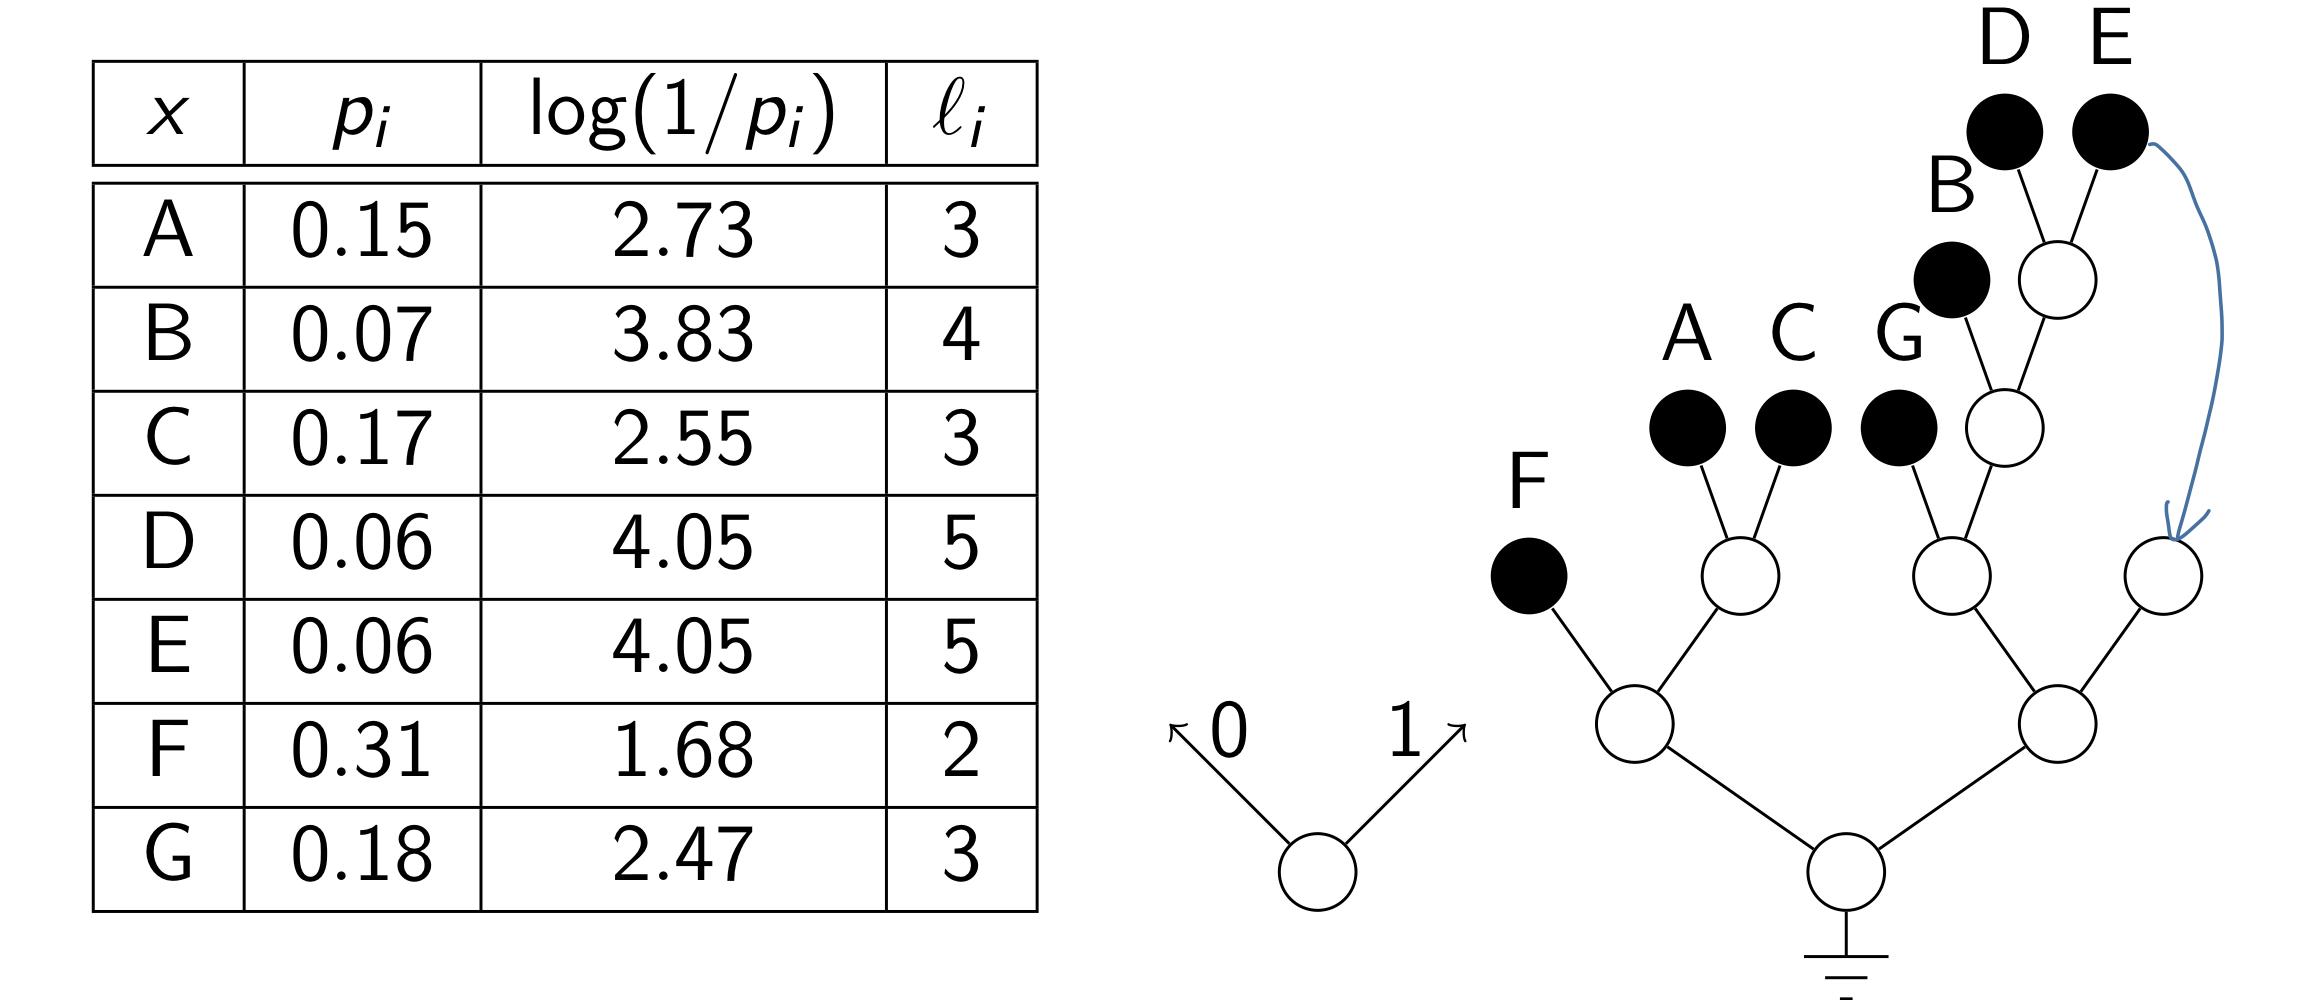
\includegraphics[width=0.8\linewidth ]{Shannon.png}
  \label{fig:1}
\end{figure}
\item Clearly, we can do better by pushing B/D/E to the length two
\end{itemize}

\subsection{Properties of Optimal prefix-free code}
\begin{enumerate}
\item The lengths are ordered inversely with the probabilities, if $p_j > p_k,$ then $\mathit{l}_j \le \mathit{l}_k$  
\item The two last probable symbols have the same length and are on neighboring leaves in the binary tree (i.e. they differ only in the last digit).
\end{enumerate}

\subsection{Huffman Coding}
\begin{itemize}
\item An algorithm gives an optimal prefix-free code for a given set of probabilities.
\begin{enumerate}
\item Take the two least probable symbols in the alphabet. these two symbols will be given the longest codewords, which will have equal length, and differ only in the last digit
\item Combine these two symbols into a single symbol, and repeat.
\end{enumerate}

\item A source produces symbols from the set \{A,B,C,D,E,F\} with probabilities \{0.05,0.1,0.15,0.2,0.2,0.3\}
\begin{enumerate}
\item List these symbols in increasing order of their probabilities.
\begin{figure}[h]
\begin{subfigure}[h]{0.3\linewidth}
  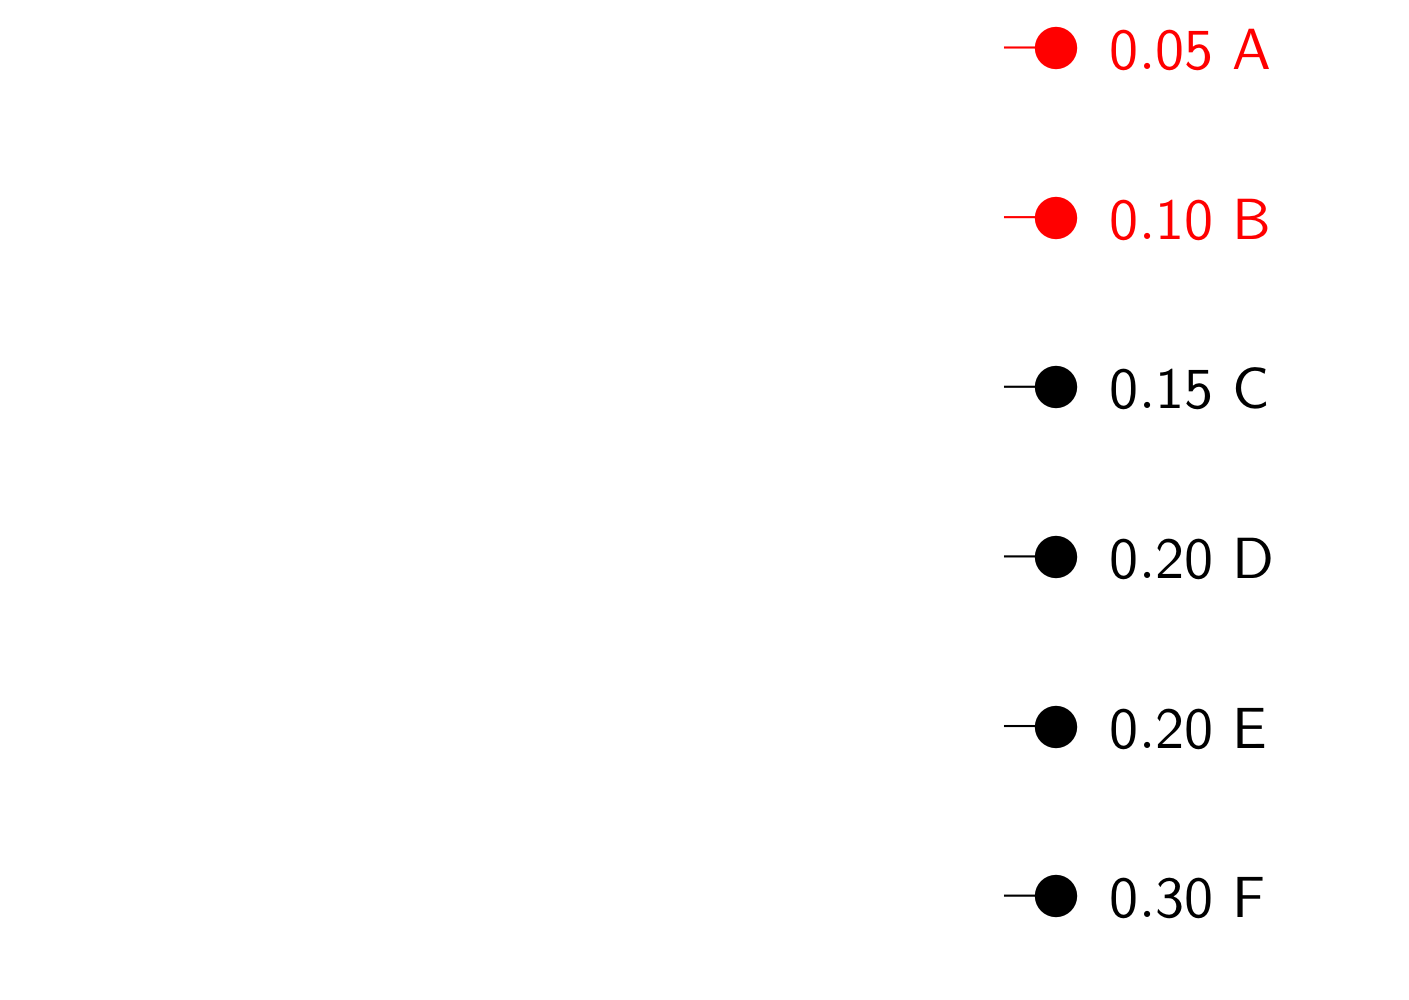
\includegraphics[width=\linewidth]{Huff1.png}
  \caption{Step 1}
\end{subfigure}
\begin{subfigure}[h]{0.3\linewidth}
  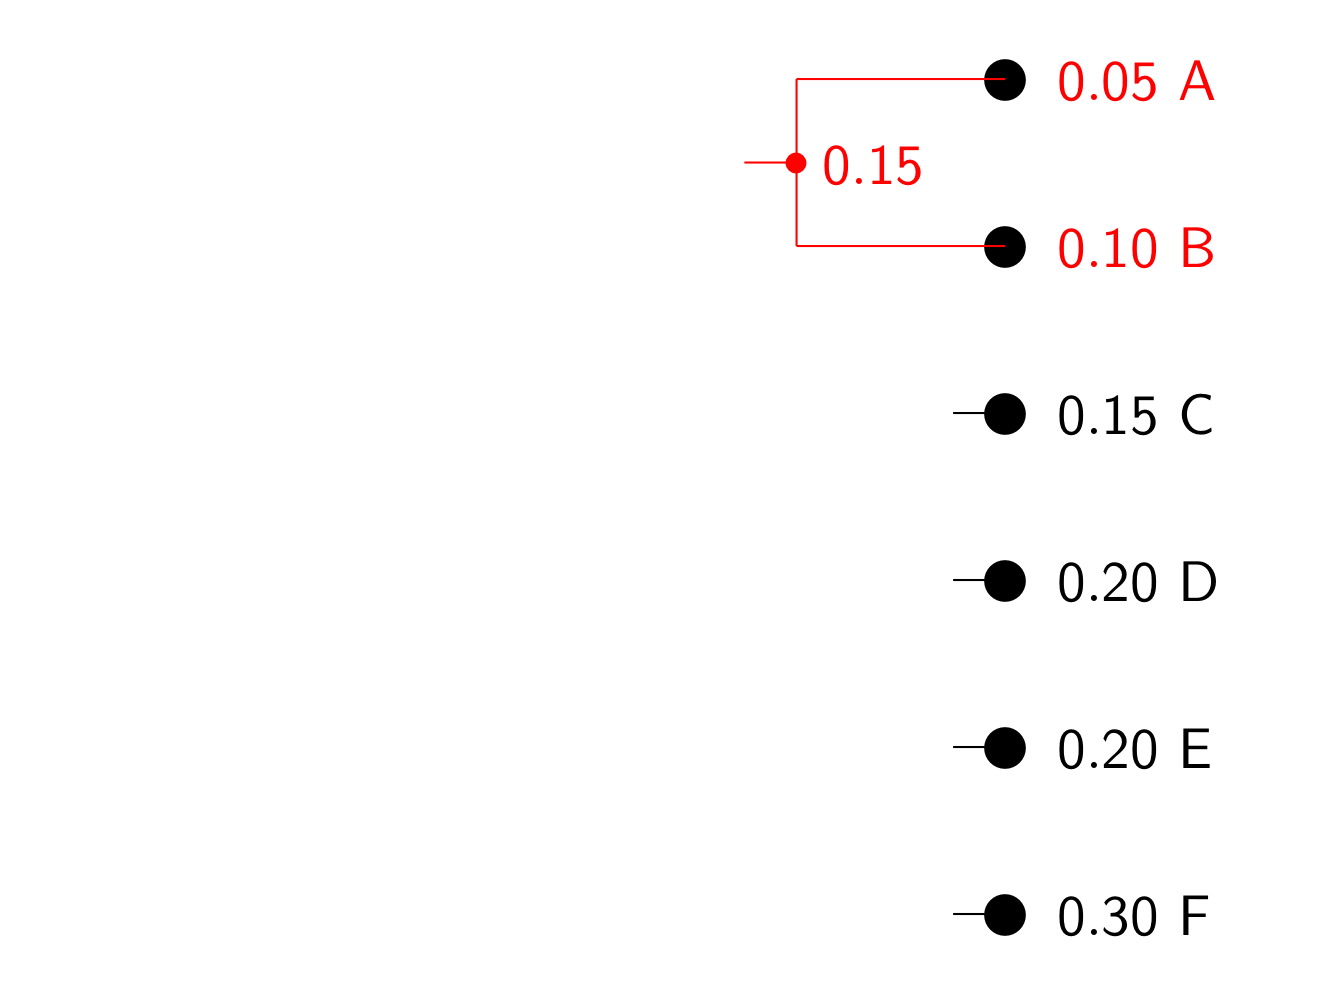
\includegraphics[width=\linewidth] {Huff2.png}
  \caption{Step 2}
\end{subfigure}
\begin{subfigure}[h]{0.3\linewidth}
  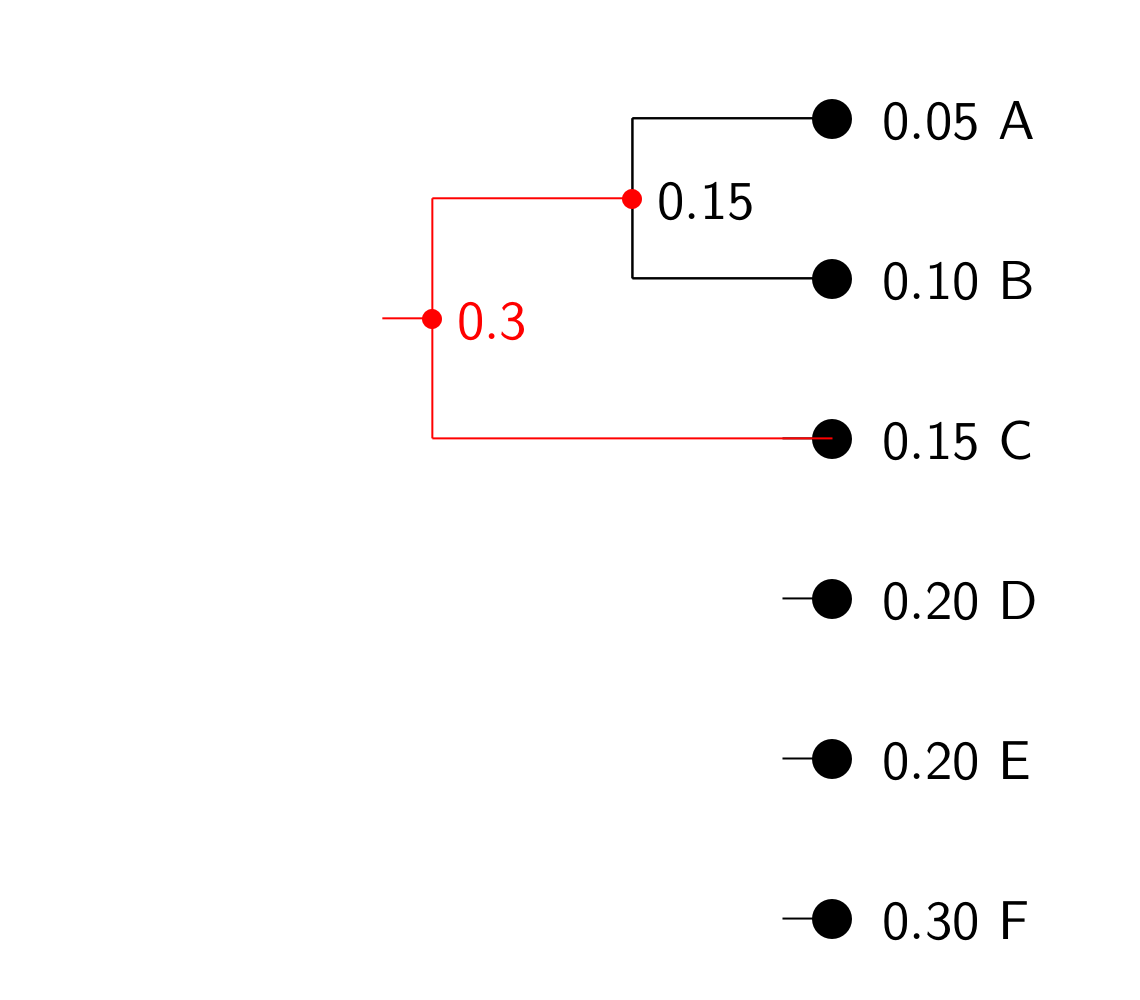
\includegraphics[width=\linewidth]{Huff3.png}
  \caption{Step 3}
\end{subfigure}
\end{figure}
\item Combine the two simple with the smallest probabilities, and form a "super-symbol" with the sum of their probabilities.

\item We now have five symbols with probabilities \{0.15,0.15,0.2,0.2,0.3\}. Again combine the two symbols with the smallest probabilities...

\item Among the four remaining symbols, D,E have the smallest probabilities, so combine
\begin{figure}[h]
\begin{subfigure}[h]{0.3\linewidth}
  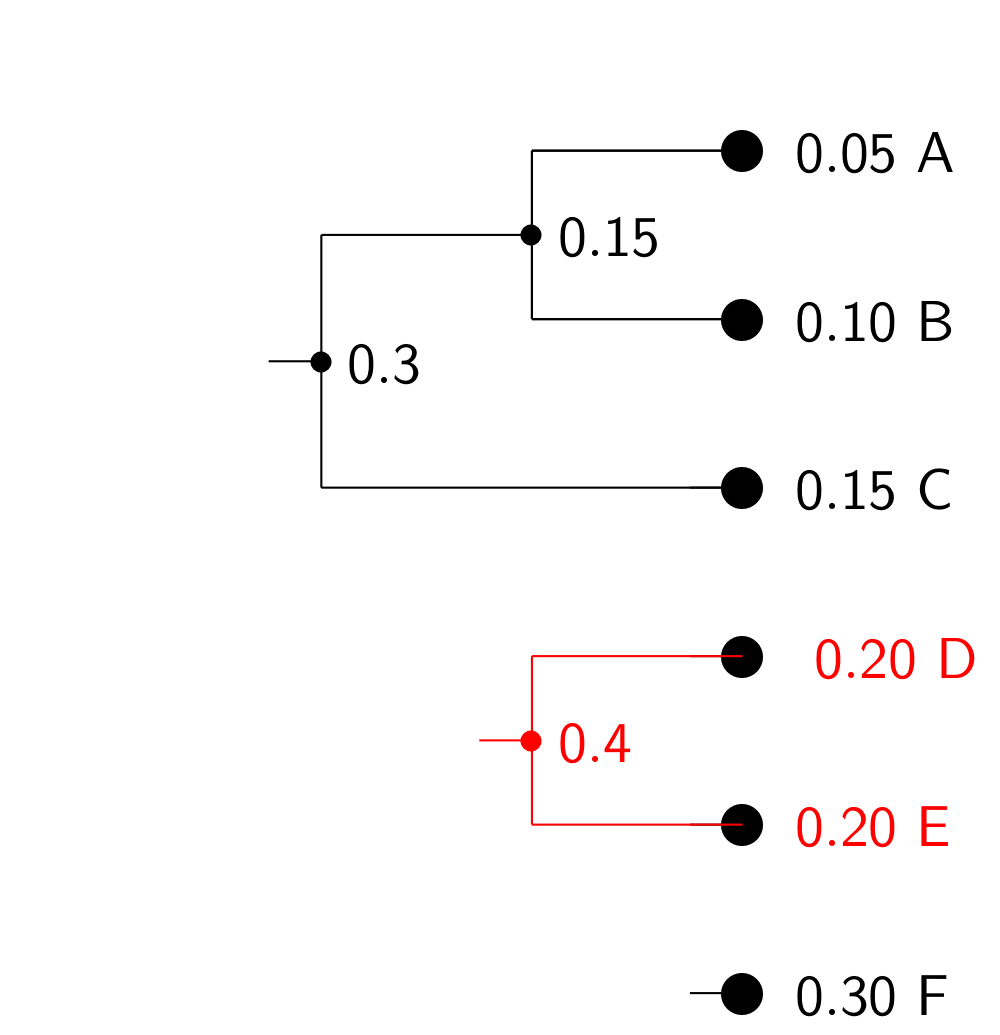
\includegraphics[width=\linewidth ]{Huff4.png}
  \caption{Step 4}
\end{subfigure}
\begin{subfigure}[h]{0.3\linewidth}
  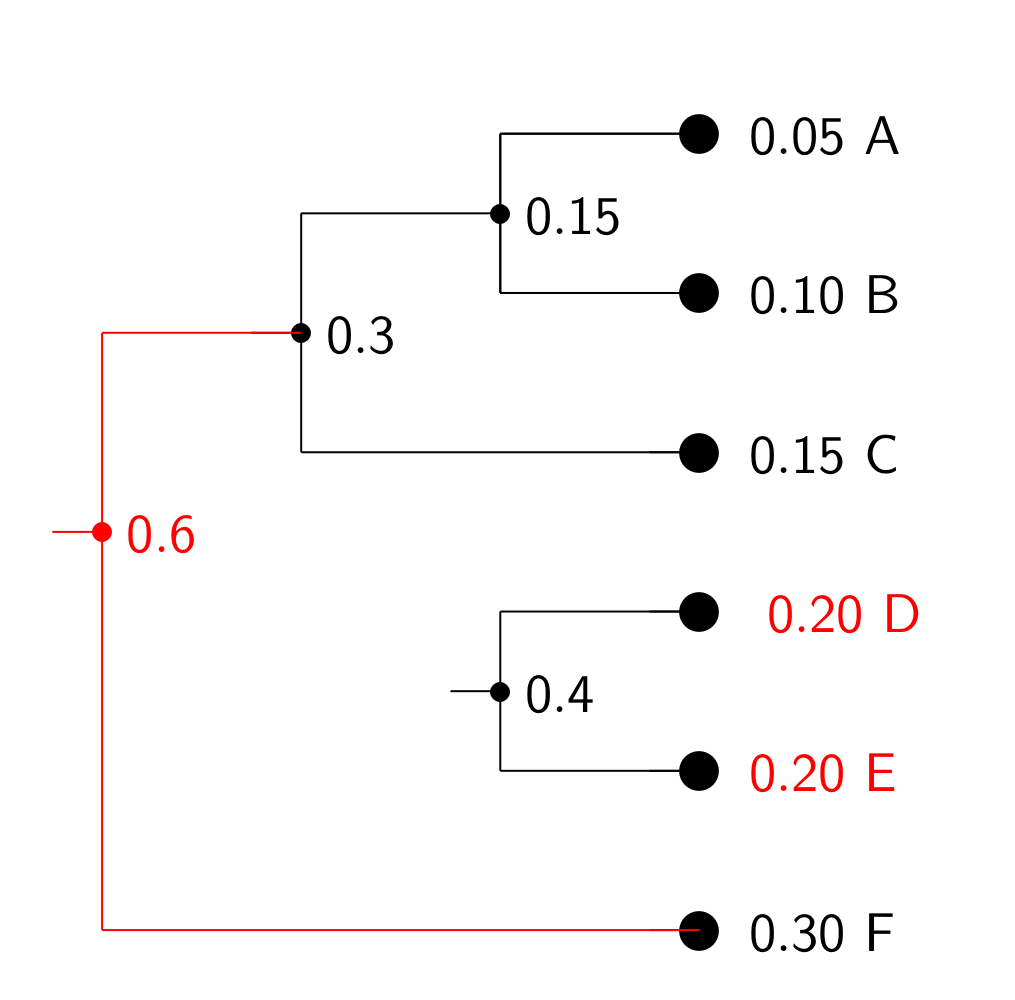
\includegraphics[width=\linewidth ]{Huff5.png}
  \caption{Step 5}
\end{subfigure}
\begin{subfigure}[h]{0.3\linewidth}
  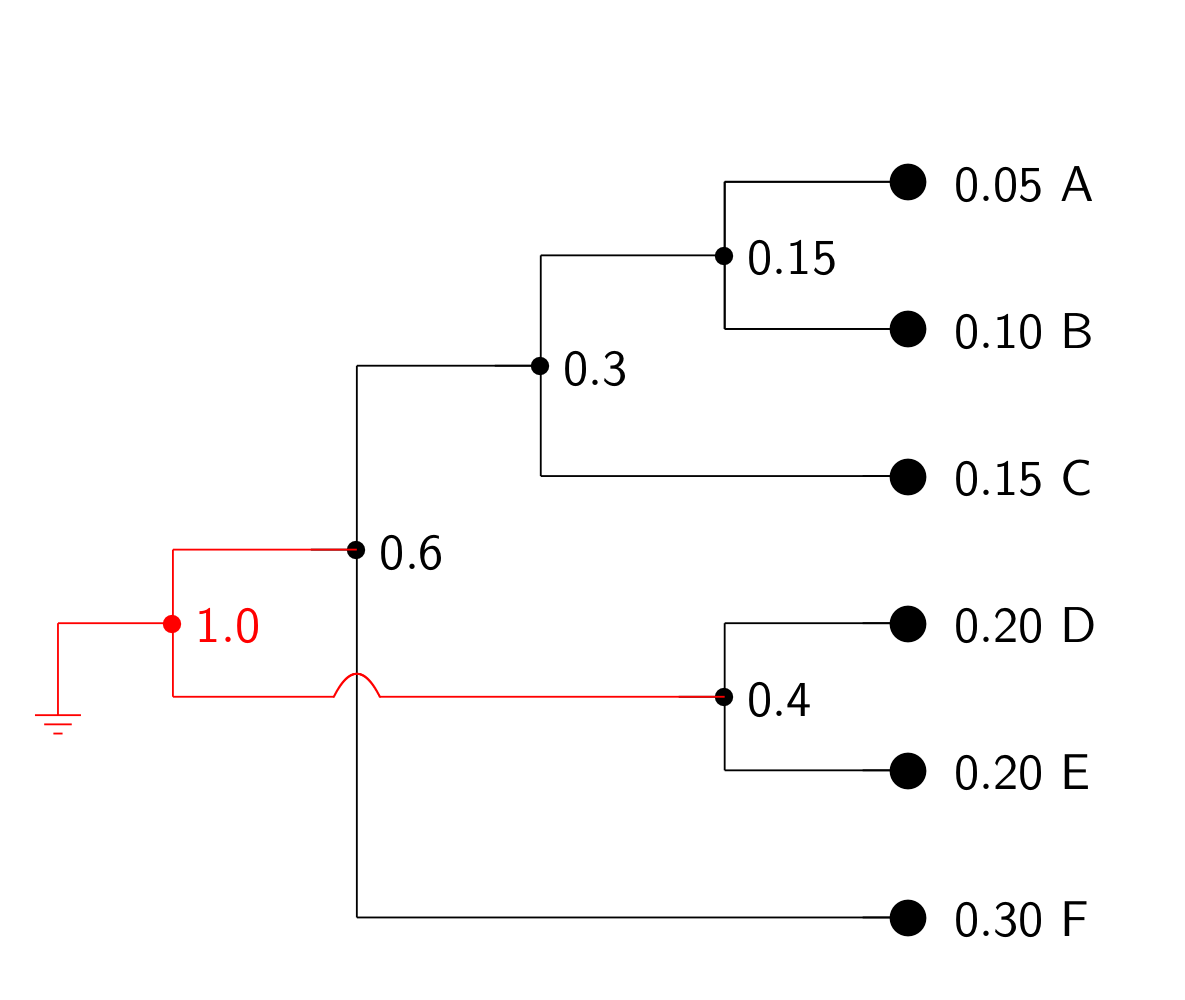
\includegraphics[width=\linewidth ]{Huff6.png}
  \caption{Step 6}
\end{subfigure}
\end{figure}
\item Among the three remaining symbols, the smallest probabilities are {0.3,0.3}, so combine them...

\item Finally, combine the remaining two symbols 

\item The symbols are the leaves of a tree. The final step is to assign the codewords to the symbols using the tree.
\begin{figure}[h]
  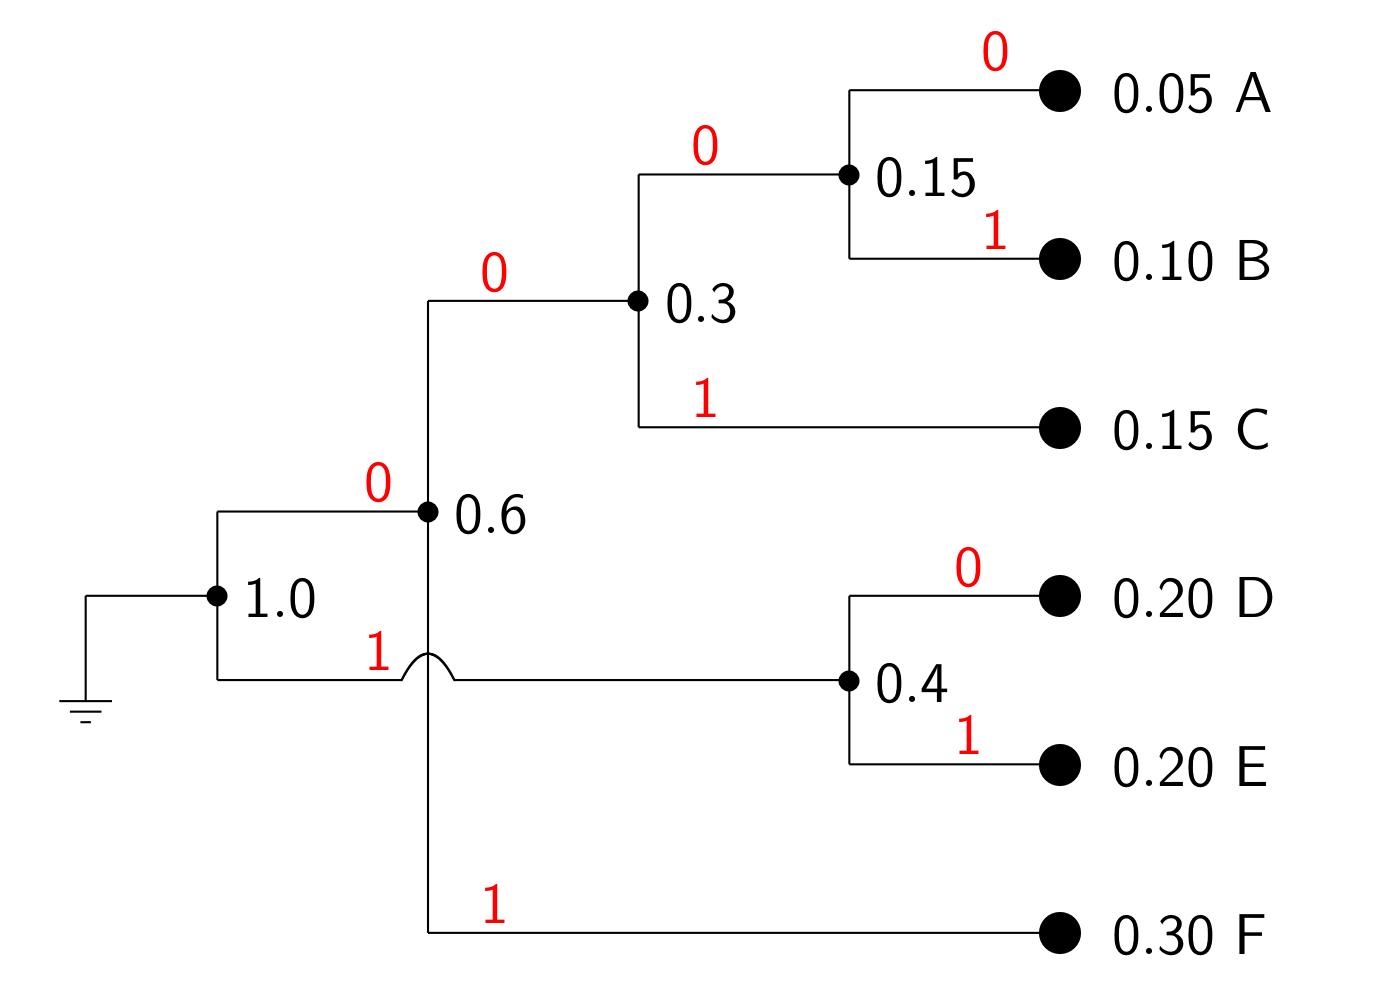
\includegraphics[width=0.3\linewidth ]{Huff7.png}
  \caption{Assign codes}
\end{figure}
\end{enumerate}
The Huffman code is:
$$F \rightarrow 01, E \rightarrow 11, D \rightarrow 10, C \rightarrow 001, B \rightarrow 0001, A \rightarrow 0000$$

\item Properties of the Huffman Code 
\begin{enumerate}
\item For a source with alphabet of size m, the Huffman algorithm requires $m-1$ steps of combining the two smallest probabilities at each stage.

\item The Huffman code for a given source may not be unique: Swapping 0/1, also 3 same prob can take any two. However, the expected code length should be the same.


\end{enumerate}
\item Optimality of Huffman coding: For a given set of probabilities, there is no prefix-free code that has smaller expected length than the Huffman code.

\item Huffman codes are optimal for coding a single random variable X, and have expected code length that is less than $H(X) + 1$ But they have some weaknesses:
\begin{itemize}
\item To reduce this overhead of up to 1 bit/symbol, we could design a Huffman code for blocks of k symbols. This would give us an overhead of 1 bit/k symbols, or 1/k bits/symbols.
\item But this comes with the expense of increased complexity. For blocks of k symbols, the binary tree is much larger.
\item These defects are addressed by Arithmetic coding, a scalable algorithm whose expected code length is very close to the source entropy for large sequences. It can also easily deal with non-iid source like text.
\end{itemize}

\end{itemize}

\subsection{Interval Coding}
\begin{itemize}
\item Key idea: Each symbol can be represented as an interval inside $[0,1]$ with length of the interval equal to the symbol probability. 

A source with m symbols with probabilities $\{ p_1,...,p_m\}$ is represented using m intervals 

\[
[0,p_1), [p_1, p_1+p_2),...,[\sum_{i=1}^{m-1}p_i, \sum_{i=1}^{m-1}p_i + p_m).
\]
\item Example: To represent interval $[0.17,0.43)$ convert the end-points to binary and find a binary interval lies completely inside this interval. say $[010,011]$ is the interval of $[0.25,0.375]$ We choose \textbf{010} as the codeword for $[0.17,0.43)$.

\item In general, the binary codeword for a symbol with probability p represented by the interval $[a,a+p)$ can be obtained as follows:
\begin{enumerate}
\item Find the largest \textit{dyadic interval} of the form $[\frac{j}{2^{\mathit{l}}}, \frac{j+1}{2^{\mathit{l}}})$ that lies within $[a,a+p)$
\item Take the binary representation of the lower end-point of the dyadic interval as the codeword.
\end{enumerate}
\item Code length: With $\mathit{l}$ code bits, the dyadic intervals have length $2^\mathit{l}$. The dyadic interval has to be contained within an interval of length p. Hence 
\[
2^\mathit{l} \le p \rightarrow \lceil \log_2(1/p) \rceil \le \mathit{l}
\]
But sometimes we'll need $\mathit{l} =\lceil \log_2(1/p) \rceil +1 $ \\
The expected code length can therefore be bounded as 
\[
L = \sum_i p_i\mathit{l}_i \le \sum_i p_i (\lceil \log_2(1/p_i) \rceil +1) < H(X) + 2
\]
\item Performance: In terms of expected code length, the analysis above shows that interval codes are in general not as good as Huffman codes or even Shannon-Fano codes. But interval coding is the basis for arithmetic coding, which is a powerful technique for long source sequences.

\end{itemize}
\subsection{Arithmetic Coding}
\begin{itemize}

\item Explain with an example. Consider a source producing symbols $X_1,X_2,...,X_n$ which are i.i.d., with each $X_i$ taking values in $\{a,b,c\}$ with probabilities $\{0.2,0.45,0.35\}$
\item Key ideas:
\begin{itemize}
\item Each length n string $(x_1,...,x_n)$ is represented by a disjoint interval with length equal to the probability of the string. 
\begin{itemize}
\item E.g. for $n=2$, $X_1=b,X_2=c$ corresponds to the probability of length $0.45 * 0.35=0.1575$ and $X_1=b,X_2=a$ of length $0.45 * 0.2=0.09$.
\end{itemize}
\item The interval for $(X_1=x,X_2=y)$ is a sub interval of the interval for $X_1=x$ 
\begin{itemize}
\item E.g. $X_1 = b$ is the interval $[0.2,0.65)$ and $(X_1 = b, X_2=c)$ is the subinterval of length $0.1575$ within  $[0.2,0.65)$ To calculate, we rewrite the interval as $\{0,0.2,0.65,0.1\}$ as the order of a,b,c.
\item The subinterval becomes $0.2 + (0.65-0.2) * 0.65 \rightarrow 0.2 + (0.65-0.2) * 1$ That is $[0.4925,0.65)$ Also we can verify that $0.65 - 0.4925 = 0.1575$
\end{itemize}  
\item Similarly, for any symbols $x,y,z$, $P(X_1=x,X_2=y,X_3=z)$ is a sub interval of $P(X_1=x,X_2=y),$ and so on.
\end{itemize}
\item Decoding: Using binary codeword to sequentially zoom in to the interval, decoding symbols as you go along.
\item Expected code length:\\
Arithmetic coding can be performed in any sequence of length n, so that any sequence $x_1,...,x_n$ can be represented by an interval of length $p(x_1,...,x_n)$, which gives a binary codeword of length at most $\lceil \log_2\frac{1}{p(x_1,...,x_n)} \rceil + 1$. \\
Therefore the expected code length for length n sequences is bounded as:
\[
L_n = \sum_{X_n} p_{x_n}\mathit{l}_{x_n} \le \sum_{x_n} p_{x_n} (\log_2\left(1/p(x_1,...,x_n)\right)+2) = H(X^n) + 2
\]
Therefore the expected code length per symbol is 
\[
\frac{L_n}{n} < \frac{H(X^n)}{n} + \frac{2}{n} = H(X) + \frac{2}{n},
\]
Where the last equality hold for $iid ~ P_X$
\end{itemize}
\subsection{Arithmetic coding for non-iid sources}
\begin{itemize}
\item Consider a source that produces symbols in alphabet $\{ a_1,...,a_m\}$ with a known distribution 
\[
P(x_1)p(x_2|x_1)...P(x_n|x_1,...,x_{n-1})
\]
The arithmetic coding algorithm can be easily extended to such sources. As before, consider the source with alphabet $\{a,b,c\}$ with probabilities $\{0.2,0.45,0.35\}$. \\
Suppose that three conditional distributions $P(X_2|X_1=a)$, $P(X_2|X_1=b)$, $P(X_2|X_1=c)$ and say
\[
P(X_2=a|X_1=b)=0.5 , P(X_2=b|X_1=b)=0.3, P(X_2=c|X_1=b)=0.2
\]
We do the same thing as before, just change the probability using the conditional probability accordingly.
\item Coding Algorithm:
\begin{itemize}
\item Let source alphabet $\mathcal{A}$ be $\{ a_1,...,a_m\}$
\item We are given a source sequence $x_1,x_2,...,x_n$ where each $x_i \in \mathcal{A}$
\item Both encoder and decoder know the conditional distributions $P_{X_1}, P_{X_2|X_1},...,P_{X_n|X_1,...,X_{n-1}}.$
\item The encoding algorithm computes the interval using the following lower and upper cumulative probabilities.
For $i=1,...m$ and for $k-1,...,n$ we define 
\[
L_k(a_i|x_1,...,x_{k-1}) = \sum_{i^{\prime}}^{i-1}  P(X_k=a_{i^{\prime}} | X_1=x_1,...,X_{k-1}=x_{k-1}) 
\]

\[
U_k(a_i|x_1,...,x_{k-1}) = \sum_{i^{\prime}}^{i}  P(X_k=a_{i^{\prime}} | X_1=x_1,...,X_{k-1}=x_{k-1})
\]
\end{itemize}
\item Finite precision issues:
The arithmetic encoding algorithm above assumes an infinite precision computer:
\begin{itemize}
\item As n grows, the length of the interval corresponding to a sequence $(x_1,...,x_n)$ shrinks
\item Hence the number of digits needed to accurately store the values lo and hi grows with n.
\end{itemize}
\end{itemize}
Summary:
\begin{enumerate}
\item Arithmetic coding can achieve compression very close to the source entropy, with complexity scaling linearly with the length of the sequence.
\item It does require you to know the conditional distribution. But this approach fits well with machine learning techniques that can mine huge quantities of text/speech/video data to build good probabilistic models.
\item Note that the assumed distribution of the source doesn't need to be true one, it only needs to be the same at both encoder and decoder.
\item Arithmetic coding works even when you generate the source conditional distribution on the fly, based on what has been observed so far. Given the generating rule, the decoder will also generate required conditional distributions as it reconstructs the sequence.
\end{enumerate}

\section{Relative Entropy Mutual Information}
\subsection{Relative Entropy}
\subsubsection{Define}
The \textbf{\textit{Relative Entropy}} or the \textit{Kullback-Leibler(KL)} divergence between two pmfs P and Q is:

\[
D(P||Q) = \sum_{x \in \rchi}P(x)\log\frac{P(x)}{Q(x)}
\]

\begin{itemize}
\item P and Q are defined on the same alphabet $\rchi$
\item Measure of distance between distributions  P and Q
\item Not a true distance. For example:  $D(P||Q) \not = D(Q||P)$
\item if $P=Q$ Then $D(P||Q) = 0$
\item Example: If $P= Bern(p) $ and $Q= Bern(q)$ for $p,q \in [0,,1],$
\[
D(P||Q) = p\log\frac{p}{q} + (1-p)\log\frac{1-p}{1-q}
\] 
\item Relative Entropy is always non-negative:
\[
D(P||Q) \ge 0 \textrm{With equality if and only if } P=Q
\]
\textit{Proof:} Using $\log_2a = \frac{\ln a}{\ln 2}$
\begin{align*}
-D(P||Q) & = \frac{1}{\ln 2} \sum_{x \in \rchi} P(x) \ln\frac{Q(x)}{P(x)} \\
& \le  \frac{1}{\ln 2} \sum_{x \in \rchi} P(x)\left( frac{Q(x)}{P(x)}\right) 
& = \frac{1}{\ln 2} (1-1) = 0
\end{align*}
Again, we use our favorite inequality $\ln x \le (x-1)$ with equality $iff$  x=1
\item We look at applications in \textcolor{blue1}{compression} and \textcolor{blue1}{hypothesis testing}.
\end{itemize}
\subsubsection{Redundancy in Source Coding}
Often the \textcolor{blue1}{True distribution} of the source is unknown, and we have to work with estimated source distribution for compression.
\begin{itemize}
\item Suppose \textcolor{blue}{true pmf} of a rv is $P = \{ p_1,...,p_m\}$, \textcolor{orange}{estimated pmf} is $\hat{P} = \{ \hat{p}_1,...,\hat{p}_m\}$
\item $\hat{P}$ is used to design a compression code whose code length $\mathit{l}_i$ satisfy
\[
\textcolor{red}{ \mathit{l}_i = \log(1/\hat{p}_i) }\qquad \textrm{for } i=1,...,m.
\]
The code is optimal for the distribution $\hat{p}$
\item How far are we from the optimal of the \textcolor{blue1}{true distribution}?
The Average code Length:
\begin{align*}
L = \sum_ip_i\mathit{l}_i & = \sum_{i}p_i \log \frac{1}{\hat{p}_i} \\
& = \sum_{i}p_i \log\frac{p_i}{p_i\hat{p}_i} \\
& = \sum_{i}p_i \log\frac{1}{p_i} + \sum_{i}p_i \log\frac{p_i}{\hat{p}_i} \\
& = H(P) + D(P||\hat{p}_i) \quad \textrm{bits/symbol}
\end{align*}
\item Therefore  $D(P||\hat{p}_i)$ is the \textcolor{red}{Price} you pay in bits/symbol --Redundancy-- for designing the code with estimated distribution rather than true distribution.

\item Example:  
Suppose we know that the true distribution $P$ is one from a set of distributions $\mathcal{P}$. For a ternary source that came from the set of distributions of the form $\mathcal{P}= \{ \gamma,0.2,0.8-\gamma\}$for $\gamma \in (0,0.8)$.

Then design a code using a distribution $\hat{P}$ that minimizes the \textit{worst-case} redundancy over this class of distribution $\mathcal{P}$, i.e.,
\[
\textrm{Choose } \hat{P} \textrm{ to minimize } \textcolor{blue1}{\max_{P\in \mathcal{P}} D(P||\hat{P})} 
\]
\[
R^* = \min_{\hat{P}} \max_{P\in \mathcal{P}} D(P||\hat{P})
\]
is called \textit{minimax} redundancy
\end{itemize}

\subsubsection{Hypothesis Testing}
We have data $X_1,...,X_n,$ and the knowledge that one of the following is true.
\[
H_0: X_1,...,X_n \textrm{ $\sim$ i.i.d. } P
\]
\[
H_1: X_1,...,X_n \textrm{ $\sim$ i.i.d. } Q
\]
Where $H_0$ is called the  \emph{null hypothesis} \vspace{1.5mm}

\textbf{Some definitions}
\begin{itemize}
    \item A decision rule or a test is a function that maps the data ($X_1,...,X_n$) to a binary decision (0 for $H_0$, 1 for $H_1$).
    \item With any decision rule, two kinds of errors can be made: \\
    \textbf{Type I error}: When $H_0$ is true, but the decision rule chooses $H_1$.\\
    \textbf{Type II error}: When $H_1$ is true, but the decision rule chooses $H_0$.
    \item Given the data $X_1,...,X_n$, the \textit{likelihood ratio}(LR) is defined as 
    \[
        \frac{Q(X_1,...X_n)}{P(X_1,...X_n)}
    \]
    and the normalized \textit{log-likelihood ratio}(LLR) is 
    \[
    \frac{1}{n}\log\frac{Q(X_1,...X_n)}{P(X_1,...X_n)}
    \]
    \item The optimum decision rule is a likelihood-ratio thresholding rule,i.e.,\\
    For some threshold T:\\
    \hspace*{10mm} Choose $H_1$ if $\frac{Q(X_1,...X_n)}{P(X_1,...X_n)} \le T$: otherwise choose $H_0$ \\
    Equivalently for LLR\\
    \hspace*{10mm} Choose $H_1$ if $\frac{1}{n}\log\frac{Q(X_1,...X_n)}{P(X_1,...X_n)} \le t$: otherwise choose $H_0$ \\
    The intuition is that Q need to comparably larger than P to be valid.\\
    Note that both tests are equivalent by setting $T= 2^{nt}$
    
    \item Increase threshold t, the condition to choose $H_1$ becomes more stringent; Hence type-I error prob. increases, type-II error prob. decreases.  
    \item If we have the optimality of thresholding tests, then: \\
    If a thresholding test has probability of Type-I error $\alpha$ and prob. of type-II error $\beta$. Then any test that lower $\alpha$ must increase $\beta$
    \end{itemize}
\textbf{Examples:} Under $H_0: X_1,...,X_n \textrm{ $\sim$ i.i.d. Bern(p)} $;  $H_1: X_1,...,X_n \textrm{ $\sim$ i.i.d. Bern(q)} $ (For Bern, 1=p or q, 0= (1-p) or (1-q)). Denote number of ones as $k_n$, we have:
\begin{align*}
    LLR(X_1,...X_n) &= \frac{1}{n}\log\frac{Q(X_1,...X_n)}{P(X_1,...X_n)}\\
                    &= \frac{1}{n}\log\frac{q^{k_n}(1-q)^{n-k_n}}{p^{k_n}(1-p)^{n-k_n}} \\
                    &= \frac{k_n}{n}\log\frac{q}{p} + \left(1- \frac{k_n}{n}\right)\log\frac{1-q}{1-p}
\end{align*}
\textbf{Question:} What is the behaviour of the LLR as n gets large when: a)  $H_0$ is true; b) $H_1$ is true
\begin{itemize}
    \item $H_0$: $X_i$ $\sim$ i.i.d. Bern(p) 
    \[
    \frac{k_n}{n} \rightarrow p \quad LLR \rightarrow p\log\frac{q}{p} + (1- p)\log\frac{1-q}{1-p} = -D(P||Q)
    \]
    \begin{itemize}
        \item When the true distribution is P, the likelihood of the data under the Q distribution(Wrong) (for large n) is 
        \[
        Q(X_1,...X_n) = P(X_1,...X_n)2^{-nD(P||Q)}
        \]
    \end{itemize}
    \item $H_1$: $X_i$ $\sim$ i.i.d. Bern(q)
    \[
    \frac{k_n}{n} \rightarrow q \quad LLR \rightarrow q\log\frac{q}{p} + (1- q)\log\frac{1-q}{1-p} = D(Q||P)
    \]
    \begin{itemize}
        \item When the true distribution is q, the likelihood of the data under the P distribution(Wrong) (for large n) is 
        \[
        P(X_1,...X_n) = Q(X_1,...X_n)2^{-nD(Q||P)}
        \]
    \end{itemize}
    \item The likelihood of the data under the wrong distribution is \textcolor{red}{\textbf{exponentially smaller}} than the likelihood under the true distribution.
    \item The exponent is controlled by the relative entropy, but note the asymmetry between $D(P||Q)$ and $(Q||P)$
\end{itemize}
    
\subsection{Mutual Information}
\begin{itemize}
    \item Consider two random variables X and Y with joint pmf $P_{XY}$. The mutual information between X and Y is defined as 
    \[
    I(X;Y) = H(X) - H(X|Y) \quad \textrm{bits}
    \]
    \item \textbf{Reduction in the uncertainty of X when you observe Y}
    \item \textbf{Property 1}
    \begin{align*}
        I(X;Y) = H(X) - &H(Y) - H(X,Y)\\
               = H(X) + &H(Y) - (H(X)+H(Y|X))\\
               = H(Y) - &H(Y|X)\\
        I(X;Y) = H(X) - &H(X|Y)\\
               = H(Y) - &H(Y|X)\\
         \textrm{X says as much about Y as Y says about X}
    \end{align*}
    \begin{figure}[h]
        \centering
        \includegraphics[width = 0.43\linewidth]{Venn_Mutual_Information.png}
        \label{fig:Venn_Mutual}
    \end{figure}
    \begin{itemize}
        \item I(X;Y) when X and Y are independent: 0 - No reduction in uncertainty
        \item I(X;Y) when Y=X: H(X) - Full reduction in uncertainty
        \item I(X:Y) when Y=f(X): H(X) - H(X|f(x)) 
    \end{itemize}
    \item \textbf{Property 2}
    \[
    I(X;Y) = D(P_{XY}||P_X P_Y)
    \]
    The relative entropy between the joint pmf and the product of the marginals \\
    Proof:
    \begin{align*}
        I(X;Y) &= H(X) - H(X|Y) \\
        &= -\sum_x P_X(x) \log P_X(x) + \sum_{x,y} \log P_{X|Y}(x|y) \\
        &= \sum_{x,y} \log \frac{P_{X|Y}(x|y)}{P_X(x)} \\
        &= \sum_{x,y} \log \frac{P_{X|Y}(x|y)P_Y(y)}{P_X(x)P_Y(y)} \\
        &= D( P_{XY} || P_X P_Y)
    \end{align*}
    
    \item \textbf{Property 3}
    \[
    I(X;Y) \ge 0
    \]
    \[
    \rightarrow H(X|Y) \le H(X), \quad H(Y|X) \le H(Y) 
    \]
    Knowing another random variable Y can only reduce the average uncertainty in X
    
    Proof: from Property 2 and $D(P||Q) \ge 0$ 
    \end{itemize}

\subsubsection{Conditional Mutual Information}
Given X, Y, Z jointly distributed according to $P_{XYZ}$, the conditional mutual information $I(X:Y|Z)$ is defined as:
\[
I([X:Y]|Z):= H(X|Z) - H(X|Y,Z).
\]
\subsubsection{Chain Rule}
For any sequence of random variables: $X_1,X_2,...,X_n$ jointly distributed with Y,
\[
I(X_1,X_2,...,X_m;Y) = \sum_{i=1}^n I(X_i;Y|X_{i-1},X_{i-2},...,X_1),
\]
By applying the conditional mutual information rule, for each i:
\[
I(X_i;Y|X_{i-1},X_{i-2},...,X_1) = H(X_i|X_{i-1},X_{i-2},...,X_1) -  H(X_i|Y,X_{i-1},X_{i-2},...,X_1)
\]

\section{Discrete Channels and Channel Capacity}

\subsection{Binary Channel}
\subsubsection{Binary Symmetric Channel(BSC)}
From Fig~\ref{fig:BSC},
\begin{align*}
    &P(Y=0|X=0) = 1 - p, &P(Y=1|X=1) = 1 - p\\
    &P(Y=1|X=0) = p, &P(Y=1|X=0) = p
\end{align*}
\begin{itemize}
    \item p is the "Crossover probability"; the channel is BSC(p)
    \item We need to find a good design of error-correcting codes for the BSC.
\end{itemize}
\begin{figure}[h]
    \centering
    \includegraphics[width=0.3\linewidth]{BSC.png}
    \caption{Binary Symmetric Channel}
    \label{fig:BSC}
\end{figure}
Example: Repetition Code
\begin{itemize}
    \item For a BSC of p=0.1, use  (1,3) repetition code:
    \begin{figure}[h]
        \centering
        \includegraphics[width=0.7\linewidth]{BSC_Rep.png}
        \caption{(1,3)Repetition coding for BSC}
        \label{fig:BSC_repti}
    \end{figure}
    \item Data bit wrongly decoded if channel flips two or more bits
    \item Probability of decoding error:$\binom 3 2 (0.1)^2(0.9) + \binom{3}{3} (0.1)^3 = 0.028$
    \item Data rate = $\frac{1}{3}$ bits/transmission
    If we apply a (1,9) or even longer repetition code:
    \item Probability of error = 0.0009 or goes to 0, but...
    \item Data rate = $\frac{1}{9} $ or $\frac{1}{n} $, which also goes to 0
\end{itemize}

\subsection{Discrete Memory less Channel}
\begin{itemize}
    \item A DMC is a system consisting of an input alphabet $ \mathcal{X}$, output alphabet $\mathcal{Y}$ and a set of transition probabilities
\[
P_{Y|X}(b|a) = Pr(Y=b|X=a) \quad \textrm{for all } a \in \mathcal{X} \textrm{ and } b \in \mathcal{Y} 
\]
\begin{figure}[h]
    \centering
    \includegraphics[width=0.3\linewidth]{DMC.png}
    \label{fig:dmc}
\end{figure}

    \item Memoryless means that the channel acts independently on each input. For each time instant $k=1,2,...$
    \[
    Pr(Y_k=y|X_k=x,X_{k-1},...,X_1,Y_{k-1},...,Y_1) = P_{Y|X}(y|x)
    \]
    \textcolor{blue1}{\textbf{Given all the past, the current output depends only on the current input}}
    
    \item Example:Binary Symmetric Channel 
    \begin{figure}[H]
    \centering
    \includegraphics[width=0.25\linewidth]{BSC.png}
    \end{figure}
    \begin{itemize}
        \item A DMC can be described by a transition probability matrix, e.g. 
    \end{itemize}
    \begin{figure}[h]
    \centering
    \includegraphics[width=0.25\linewidth]{DMC_BSC.png}
    \end{figure}
    
    \item Example: Binary Erasure Channel (BEC):
    \begin{figure}[h]
    \centering
    \includegraphics[width=0.5\linewidth]{DMC_BEC.png}
    \end{figure}
\begin{itemize}
    \item Erasure can model packet loss in networks
    \item When the demodulator thinks the output symbol is too noisy, it can declare an erasure
\end{itemize}
\item Noisy Keyboard Channel: A useful toy example 
\begin{figure}[h]
    \centering
    \includegraphics[width=0.25\linewidth]{Keyboard_Channel.png}
\end{figure}
\begin{itemize}
    \item Input alphabet of 26
    \item Each channel input is either received unchanged or transformed into next symbol:
    \begin{align*}
        P(Y=a|X=a) &= P(Y=b|X=a) = \frac{1}{2}, \\
        P(Y=b|X=b) &= P(Y=c|X=b) = \frac{1}{2}, \\
        &\vdots \\
        P(Y=z|X=z) &= P(Y=a|X=z) = \frac{1}{2} \\
    \end{align*}
\end{itemize}
To achieve error-free over this channel:
\begin{figure}[h]
    \centering
    \includegraphics[width=0.4\linewidth]{Keyboard_Errorlesss.png}
\end{figure}
\begin{itemize}
    \item Use only symbols a,c,e,...,y
    \item Noiselessly convey one of 13 symbols per transmission
    \item $\Longrightarrow$ Transmission rate = $\log 13$ bits/transmission
    \item This is in fact the maximum possible rate
\end{itemize}
\end{itemize}
For a general DMC:
\begin{itemize}
    \item Construct a set of input sequences which have \textcolor{red}{\textbf{Non-Intersecting }} sets of output sequences with high probability
    \item These input sequences are non-confusable as to the inputs a,c,e... in the keyboard channel.
\end{itemize}
\subsection{Channel Capacity}
\begin{figure}[h]
    \centering
    \includegraphics[width=0.25\linewidth]{Channel_Capacity.png}
\end{figure}
\centerline{\large The channel capacity of a discrete memoryless channel is defined as }

\[
C = \max_{P_X}I(X;Y)
\]
\begin{itemize}
    \item $P_{Y|X}$ is defined by the DMC. Each input distribution $P_X$ yields a differeent joint distribution on (X,Y) given by $P_X P_{Y|X}$
    \item C is the maximum transmission rate over the DMC for arbitrarily small probability of error
    
\end{itemize}
Example 1: Noiseless Binary Channel 
\begin{figure}[H]
    \centering
    \includegraphics[width=0.3\linewidth]{L7/Noiseless_BC.png}
\end{figure}
\[
I(X;Y) = H(X) - H(X|Y) = H(X) \quad (H(X|Y)=0)
\]
\begin{itemize}

\item Channel capacity is maximize mutual information, so here maximize H(X) $\rightarrow P_X=(\frac{1}{2},\frac{1}{2})$
\item Therefore
\[
C = \max_{P_X}I(X;Y) = \max_{P_X}H(X) = 1 \textrm{bit/transmission}
\]
\end{itemize}

Example 2: BSC
\begin{figure}[H]
    \centering
    \includegraphics[width=0.25\linewidth]{BSC.png}
\end{figure}
\begin{align*}
    I(X;Y) &= H(Y) - H(Y|X) \\
    & = H(Y) - \sum_{x\in {0,1}}P_X(x)H(Y|X=x)\\
    & = H(Y) - \sum_{x\in {0,1}}P_X(x)H_2(P)\\
    & = H(Y) - H_2(P)\\
    & \le 1 - H_2(P)
\end{align*}
\begin{itemize}
    \item $H(Y|X=x)=H_2(P)$ since $H(Y|X=0) = H((Y|X=1) = H\{1-p,p\} = H\{p,1-p\}$
    \item Maximum value of H(Y) = 1 is attained when $P_X=(0.5,0.5) \rightarrow C=1-H_2(p)$
    \item For p = 0.1, C = 0.531 bits/transmission
\end{itemize}

Example 3 : Noisy Keyboard Channel

\begin{figure}[h]
    \centering
    \includegraphics[width=0.25\linewidth]{Keyboard_Channel.png}
\end{figure}
\begin{align*}
    I(X;Y)& = H(Y)- H(Y|X)
    & = H(Y) - 1 \le \log(26) - 1 = \log(13)
\end{align*}

\begin{itemize}
    \item what $P_X$ maximises $H(Y)$?  We have two choices!
    \begin{enumerate}
        \item $P_X = (1/26,...,1/26)$
        \item $P_X = (1/13,0,...,1/13,0)$ [We used before]
    \item Both yield $P_Y=(1/26,1/26,...,1/26)$
    \[
    C = \max_{P_X}I(X;Y) = \log(26) - 1 = \log(13) \textrm{ bits/transmission}
    \]
    \end{enumerate}
\end{itemize}
\section{Channel Coding Theorem}

{\large \textbf{Definition of a Channel Code}}
\begin{figure}
    \centering
    \includegraphics[width=0.3\linewidth]{L7/Channel_code.png}
\end{figure}
\begin{itemize}
    \item We use the channel n times to transmit k information bits.
    \item Each sequence of k-bits as indexing a ``message'' W in the set $\{1,...,2^k\}$ \\
    k bits $\Leftrightarrow$ $2^k$ messages
    \item The rate R of the code is $R=\frac{k}{n}$ bits/transmission. Then the total number of messages is $2^k = 2^{nR}$.
\end{itemize}
An (n,k) channel code of rate R for the channel $(\mathcal{X}, \mathcal{Y}, P_{Y|X})$ consists of:
\begin{enumerate}
    \item A set of messages: $\{1,...,2^k=2^{nR}\}$
    \item an \textcolor{red}{encoding} function $X^n$: $\{1,...,2^k\} \rightarrow \mathcal{X}^n$ that assigns a \textcolor{blue1}{\textbf{codeword}} to each message. The set of codewords $\{X^n(1),...,X^n(2^{nR})\}$ is called the \textcolor{blue1}{\textbf{codebook}}
    \item A \textcolor{red}{decoding} function g: $\mathcal{Y}^n \rightarrow \{1,...,2^{nR} \}$, which produces a guess of the transmitted message for each received vector
\end{enumerate}

\subsection{Preview of Channel Coding Theorem}
\begin{figure}[H]
    \centering
    \includegraphics[width=0.3\linewidth]{L7/BSC01.png}
\end{figure}
For BSC(0.1):
\begin{itemize}
    \item For input sequence $X^n$, the output $Y^n $ is generated as 
    \[
    Y_i = X_i \oplus E_i \quad \textrm{for } i = 1,...,n
    \]
    \item Note:
    \[
    X_i \oplus 0 = X_i \qquad X_i \oplus 1 = \Bar{X}_i
    \]
    \item $E_1,...,E_n$ i.i.d $\sim$ Bern(0.1) is the sequence of errors introduced by the channel
    \item For large n, the number of ones in $(E_1,...,E_n) \simeq 0.1n$ (AEP)
\end{itemize}
{\large \textbf{How big is the set of $Y^n$ sequences ``typical'' with any given $X^n$? }}
\[
2^{n H_2(0.1)}
\]
\begin{figure}[H]
    \centering
    \includegraphics[width=0.6\linewidth]{L7/Typical_Sequence.png}
\end{figure}
\begin{itemize}
    \item the high-probability set of typical $Y^n$ Sequences for a given $X^n(1)$ is much smaller than $2^n$
    \item pick $X^n(2)$ far enough away from $X^n(1)$.
    \item Then the typical set of $Y^n$'s for $X^n(2)$ is non-intersecting with the typical set for $X^n(1)$. This could again carried out for  $X^n(3)....$
    \item Number of distinct messages we can transmit = max.number of non-intersecting sets .
    \[
    2^{nR} \simeq \frac{2^n}{2^{nH_2(0.1)}} \Rightarrow \textrm{ Rate R} \simeq 1 - H_2 0.1) = \textrm{Channel Capacity}
    \]
\end{itemize}
\subsection{General DMC} 
Fix an input pmf $P_X$. Together with the channel $P_{Y|X}$, this gives 
\[
P_{XY} = P_X P_{Y|X} P_Y = \sum_X P_X P_{Y|X}
\]

If $X^n(1),X^n(2),...,X^n(2^{nR})$ are generated i.i.d $\sim$ $P_X$, then:
\begin{itemize}
    \item When $X_n(j)$ is transmitted, the set of highly likely $Y_n$'s has approximately $2^{nH(Y|X)}$ sequences for each $j\in \{ 1,...,2^{nR}\}$
    \item These sets are non-intersecting with high probability
    \begin{figure}[H]
        \centering
        \includegraphics[width=0.6\linewidth]{L7/General_DMC.png}
    \end{figure}
\end{itemize}

\subsection{Joint typicality}
Example: Let$(X^n,Y^n)$ be drawn i.i.d. according to the following joint pmf: 
\begin{figure}[H]
    \centering
    \includegraphics[width=0.25\linewidth]{L7/Jointtypical.png}
\end{figure}
\[
Pr(X_n = x^n, Y^n = y^n) = \prod_{i-1}^n P_{XY}(x_i,y_i), \quad \textrm{for all }(x^n,y^n).
\]
For large n,
\begin{itemize}
    \item $X^n$ and $Y^n$ will each have approximately $50\%$ ones.
    \item The number of $(X_i,Y_i)$ pairs that are $(0,0),(0,1),(1,0),(1,1)$ will be close to $.4n,.1n,.1n,.4n$.
\end{itemize}

\subsection{Joint Typical Set}
The set $A_{\epsilon,n}$ pf \textcolor{blue1}{\textit{jointly typical}} sequences $\{ (x^n, y^n)\}$ with respect to a joint pmf $P_XY$ is defined as 
\begin{align*}
    A_{\epsilon,n} = \{ &(x^n, y^n) \in \mathcal{X}^n \times \mathcal{Y}^n \textrm{ such that} \\  
    &|- \frac{1}{n} \log P_X(x^n)-H(X)| < \epsilon\\
    &|- \frac{1}{n} \log P_Y(y^n)-H(Y)| < \epsilon\\
    &|- \frac{1}{n} \log P_{XY}(x^n,y^n)-H(X,Y)| < \epsilon \}
\end{align*}
Where $P_{XY}(x^n,y^n) = \prod_{i=1}^N P_{XY}(X_i,y_i)$

\begin{figure}[H]
    \centering
    \includegraphics{L7/JointTypicalSet.png}
\end{figure}

\subsection{Joint AEP}
{\large{AEP: \textit{Asymptotic equipartition property}}}\\
Let $(X_n,Y_n)$ be a pair of sequences drawn i.i.d. according to $P_{XY}$, i.e.,
\[
Pr(X^n=x^n,Y^n=y^n) = \prod_{i=1}^n P_{XY}(X_i,y_i), \quad \textrm{for all }(x^n,y^n)
\]
Then for any $\epsilon > 0$:
\begin{enumerate}
    \item $Pr((X^n,Y^n)\in A_{\epsilon ,n}) \rightarrow 1$ as $n\rightarrow \infty$
    \item $|A_{\epsilon , n}| \le 2^{n(H(X,Y)+\epsilon)}$  (Size of typical set)
    \item If $(\Tilde{X}^n,\Tilde{Y}^n)$ are a pair of sequences drawn i.i.d according to $P_X P_Y$ [i.e. $\Tilde{X}^n,\Tilde{Y}^n$ are independent with the same marginals as $P_{XY}$], then 
    \[
    Pr((\Tilde{X}^n,\Tilde{Y}^n)\in A_{\epsilon ,n}) \le 2^{-n(I(X;Y)-3\epsilon)}
    \]
\end{enumerate}
\subsection{Proof of AEP}
\subsubsection{Claim 1:}
When $(X_n,Y_n)$ drawn i.i.d. according to $P_{XY}$,
\begin{align*}
    &Pr\left(|- \frac{1}{n} \log P_X(x^n)-H(X)| < \epsilon \right) \rightarrow 1 \textrm{ as } n\rightarrow\infty\\
    &Pr\left(|- \frac{1}{n} \log P_Y(y^n)-H(Y)| < \epsilon \right) \rightarrow 1 \textrm{ as } n\rightarrow\infty\\
    &Pr\left(|- \frac{1}{n} \log P_{XY}(x^n,y^n)-H(X,Y)| < \epsilon \right) \rightarrow 1 \textrm{ as } n\rightarrow\infty 
\end{align*}
The proof of the above is very similar to that of the AEP in Handout 2 and follows from the WLLN. Thus $Pr((X^n,Y^n)\in A_{\epsilon ,n}) \rightarrow 1$ as $n\rightarrow \infty$
\subsubsection{Claim 2:}
We have 
\begin{align*}
    1 &= \sum_{x^n,y^n}P_{XY}(x^n,y^n)\\
    &\ge \sum_{(x^n,y^n)\in A_{\epsilon ,n}}P_{XY}(x^n,y^n)\\
    & \ge \sum_{(x^n,y^n)\in A_{\epsilon ,n}} 2^{-n(H(X,Y)+\epsilon)}\\
    & = 2^{-n(H(X,Y)+\epsilon)}|A_{\epsilon,n}|
\end{align*}
Hence $|A_{\epsilon,n}| \le 2^{n(H(X,Y)+\epsilon)}$. 

\subsubsection{Claim 3:}
If $(\Tilde{X}^n,\Tilde{Y}^n)$ are independent but have the same marginals as $X^n$ and $Y^n$, then 
\begin{align*}
    Pr((\Tilde{X}^n,\Tilde{Y}^n)\in A_{\epsilon ,n}) &= \sum_{(x^n,y^n)\in A_{\epsilon ,n}}P_X(x^n)P_Y(y^n) \\
    &\le 2^{n(H(X,Y)+\epsilon)} \cdot 2^{-n(H(X)-\epsilon)} \cdot 2^{-n(H(Y)-\epsilon)} \\
    &= 2^{-n(I(X;Y)-3\epsilon)}
\end{align*}
\begin{figure}[H]
    \centering
    \includegraphics[width=0.7\linewidth]{L7/Claim3.png}
\end{figure}
\subsection{The probability of Error of a code}
\begin{figure}[H]
    \centering
    \includegraphics[width=0.5\linewidth]{L7/Error.png}
\end{figure}
The \textit{maximal} probability of error of the code is defined as 
\[
\max_{j\in \{1,...,2^{nR}\}} Pr(\hat{W}\not = j | W=j)
\]
The \textit{average} probability of error of the code is
\[
\frac{1}{2^{nR}} \sum_{j=1}^{2^{nR}} Pr(\hat{W}\not = j | W=j)
\]
$W$ and $\hat{W}$ denote the transmitted, and decoded messages respectively.

\subsection{The Channel Coding Theorem}
{\large \textit{For a DMC with capacity C, all rates less than C are achievable.}}.
\begin{enumerate}
    \item Fix $R<C$ and pick any $\epsilon > 0$. Then, for all sufficiently large n there exists a length-n code of rate R with maximal probability of error less than $\epsilon$
    \item Conversely, any sequence of length-n codes of rate R with average/maximal probability of error $P_e^{(n)} \rightarrow 0$ as $n\rightarrow \infty$ must have $R \le C$.
\end{enumerate}
\subsubsection{Proof of the coding theorem}
Prove the achievability of all rates $R<C$. (the first part).\\
{\large \textcolor{blue1}{\textit{Codebook Generation:}}}
\begin{itemize}
    \item Fix rate $R<C$ and input pmf $P_X$. We generate each of the $2^{nR}$ codewords independently according to the distribution
    \[
    Pr(X_n(k) = (x_1,...,x_n)) = \prod_{i=1}^n P_X(x_i)\quad \textrm{for } k=1,...,2^{nR}.
    \]
    \item Codebook $\mathcal{B}$ can be interpreted as a $2^{nR} \times n$ matrix:
        
        \[
        \mathcal{B}
        =
        \begin{bmatrix}
        X_1(1) & X_2(1) & \cdots& X_n(1) \\
        X_1(2) & X_2(2) & \cdots& X_n(2) \\
        \vdots & \vdots & \ddots& \vdots \\
        X_1(2^{nR}) & X_2(2^{nR}) & \cdots& X_n(2^{nR}) \\
        \end{bmatrix}
        =
        \begin{bmatrix}
        \textrm{Length n codeword - Message }1 \\
        \textrm{Length n codeword - Message }2 \\
        \vdots \\
        \textrm{Length n codeword - Message }2^{nR} \\
        \end{bmatrix}
        \]
        

    \item Each entry in the matrix is chosen i.i.d according to $P_X$. The probability that we generate a particular codebook $x^n(1),...,x^N(2^{nR})$ is $\prod_{w=1}^{2^{nR}}\prod_{i=1}^n P_X(x_i(w))$
\end{itemize}

\subsubsection{Encoding}\begin{figure}[H]
    \centering
    \includegraphics[width=0.5\linewidth]{L7/Error.png}
\end{figure}
\begin{enumerate}
    \item A codebook $\mathcal{B}$ is generated as described previously. The codebook is revealed to both sender and receiver, who also know the channel transition matrix $P_{Y|X}$.
    \item To transmit message $W$, the encoder sends $X^n(W)$ over the channel 
    \item The receiver receives a sequence $Y^n$ generated according to 
    \begin{equation}
        \prod_{i=1}^n P_{Y|X}(Y_i|X_i(W))
        \label{eq:Encoded_Received}
    \end{equation}
    \item From $Y^n$, the receiver has to guess which message was sent.
    \begin{itemize}
        \item Assuming a uniform prior on the messages, the optimal decoding rule is max-likelihood decoding: decode the message $\hat{W}$ that maximises Eq.~\ref{eq:Encoded_Received}
        \item But \textit{\textcolor{blue1}{joint typical }}decoding is used for easier analyze.
    \end{itemize}
\end{enumerate}
\subsubsection{Joint Typicality Decoder}
The decoder declares that the message $\hat{W}$ was sent if both the following conditions are satisfied:
\begin{itemize}
    \item $(X^n(\hat{W}), Y^n)$ is jointly typical with respect to $P_X P_{Y|X}$.
    \item There exists no other message $W\prime \not = \hat{W}$ such that  $(X^n(\hat{W}), Y^n)$ is jointly typical.
\end{itemize}
If no such $\hat{W}$ is found or there is more than one such, an error is declared.
\subsubsection{Analyze the probability of error}
\begin{itemize}
    \item The average probability of error for a given codebook $\mathcal{B}$ is 
    \begin{equation}
        \frac{1}{2^{nR}} \sum_{w=1}^{2^{nR}} Pr(\hat{W}\not = w |\mathcal{B}, W=w)
        \label{eq:average_error}
    \end{equation}
    \item Analysing this for a specific codebook is hard. So the average of Eq.~\ref{eq:average_error} over all codebooks is calculated:
    \begin{align*}
        \Bar{P}_e &= \frac{1}{2^{nR}} \textcolor{red}{\sum_{\mathcal{B}}}\sum_{w=1}^{2^{nR}} Pr(\hat{W}\not = w |\mathcal{B}, W=w)\textcolor{red}{Pr(\mathcal{B})}. \\
        \Bar{P}_e &= \frac{1}{2^{nR}} \sum_{w=1}^{2^{nR}} \textcolor{red}{\sum_{\mathcal{B}}} Pr(\hat{W}\not = w |\mathcal{B}, W=w)\textcolor{red}{Pr(\mathcal{B})}. \\
    \end{align*}
    \item Recall $Pr(\mathcal{B})$ is the probability corresponding to picking each symbol of $\mathcal{B}$ i.i.d. $\sim$ $P_X$.
    \item Since all the messages are equally likely, we can assume that the first message is the transmitted one. Thus
    \[
    \Bar{P}_e =  \sum_{\mathcal{B}}  Pr(\hat{W}\not = 1 |\mathcal{B}, W=1)Pr(\mathcal{B}). 
    \]
\end{itemize}
\subsubsection{Error Analysis}
Assuming W=1 was transmitted, there are two sources of error:
\begin{enumerate}
    \item $X^n(1)$ is not jointly typical with the output $Y^n$.
    \item $X^n(k)$ is jointly typical with the output $Y^n$ for some $k \not = 1$.
\end{enumerate}
\begin{itemize}
    \item Let $E_k$ be the event that $X_n(k)$ and $Y^n$ are jointly typical.
    \item Then:
    \begin{align*}
        \Bar{P}_e =& P(E_1^C \cup E_2 \cup ... \cup E_{2^nR})\\
        \le & P(E_1^C) + P(E_2) + ... + P(E_{2^nR}) \\
        &\textrm{(Union Bound)}
    \end{align*}
\end{itemize}
1) Showing $P(E_1^C)$ is small:
\begin{itemize}
    \item $X^n(1)$ i.i.d. $\sim P_X$.
    \item The channel generates $Y^n$ symbols by symbol according to $P_{Y|X}(Y_i|X_i(1))$ for $i=1,...,n$
    \item Therefore $X^n(1), Y^n$ is generated i.i.d $\sim P_X P_{Y|X}$
    \item Joint AEP implies that $P(E_1^C) \le \epsilon$ for sufficiently large n 
\end{itemize}
2) Showing $ P(E_2) + ... + P(E_{2^nR})$ is small:

For $k\not = 1$:
\begin{itemize}
    \item $X^n(k)$ was generated independently from $X^n(1)$, and $Y^n$ is obtained by passing $X^n(1)$ through the channel. 
    \item Hence $X^n(k)$ and $Y^n$ are independent for $k \not = 1$.
    \item Further, $X^n(k)$ is i.i.d. $\sim P_X$, and $Y^n$ is i.i.d. $\sim P_Y$.
    \item From the Joint AEP, the probability that $X_n(k)$ and $Y_n$ are jointly typical according to $P_{XY}$ is $\le 2^{-n(I(X;Y)-3\epsilon)}$
    \[
    \Rightarrow P(E_2)+...+ P(E_{2^nR}) \le (2^{nR}-1)2^{-n(I(X;Y)-3\epsilon)}
    \]
    Putting the two parts together:
    \begin{align*}
        \Bar{P}_e &\le P(E_1^C) + P(E_2) +...+ P(E_{2^{nR}})\\
        &\le \epsilon + 2^{nR}2^{-n(I(X;Y)-3\epsilon)} \\
        &\le^{(a)} \epsilon + \epsilon
    \end{align*}
    (a) is true when $R<I(X;Y)-3\epsilon$ and n is sufficiently large.
    \end{itemize}
Therefore combining 1) and 2):
\[
\Bar{P}_e = \frac{1}{2^{nR}} \sum_{w=1}^{2^{nR}} {\sum_{\mathcal{B}}} Pr(\hat{W}\not = w |\mathcal{B}, W=w){Pr(\mathcal{B})} \le 2\epsilon 
\]
{\Large \textbf{Final Steps:}}
\begin{enumerate}
    \item Choose $P_X$ to be one that maximises $I(X;Y)$.
    \item Get rid of average over codebooks:  As $\Bar{P}_e \le 2\epsilon$, there exists at least one codebook $\mathcal{B}*$ with
    \[
    P_e(\mathcal{B}^*) = \frac{1}{2^{nR}} \sum_{w=1}^{2^{nR}} Pr(\hat{W}\not = w |\mathcal{B}^*, W=w){Pr(\mathcal{B})} \le 2\epsilon 
    \]
    \item Throw away the worst half of the codewords in $\mathcal{B}^*$: For $\mathcal{B}^*$, the probability of error averaged over all messages is $\le 2\epsilon$. Thus the probability of error must be $\le 4\epsilon$ for at least halt the messages.
\end{enumerate}
    
\subsubsection{The Final Code}
\begin{itemize}
    \item The number of codewords in this improved version of $\mathcal{B}^*$ is $2^{nR}/2$. Its rate is 
    \[
    \frac{\log(2^{nR}/2)}{n}=R- \frac{1}{n}.
    \]
    \item Since R is any rate less than $C-3\epsilon$, we have shown the existence of a code with rate 
    \[
    C - 4\epsilon -\frac{1}{n}
    \]
    whose maximal probability of error satisfies 
    \[
    \max_{W} Pr(\hat{W}\not = w | W=w) \le 4\epsilon
    \]
    \item Since $\epsilon >0$ is an arbitrary constant, we have shown that for any $R<C$, for sufficiently large n there exists a code with arbitrarily small maximal error probability. 
    \item This proves the first part of channel coding theorem, the converse would be proved in next chapter.
\end{itemize}
\subsection{Summary}
\begin{itemize}
    \item Allow an arbitrarily small but non-zero probability of error
    \item Use the channel many times in succession, so that the law of large numbers comes into effect
    \item Random Coding: Calculate the average probability of error over a random choice of codebooks, which can then be used to show the existence of at least one good code
\end{itemize}




\newpage
\section{Data Processing, Fano's Inequality}
\subsection{Data Processing and Mutual Information}
\begin{figure}[H]
    \centering
    \includegraphics[width=0.5\linewidth]{L8/Processor.png}
\end{figure}
Random variables, X,Y,Z are said to form a \textcolor{blue1}{\textbf{Markov chain}} if their joint pmf can be written as 
\[
P_{XYZ} = P_XP_{Y|X}P_{Z|Y}
\]
In other words, the conditional distribution of Z given (X,Y) depends only on Y, i.e., $P_{Z|XY} = P_{Z|Y}$.
Example of Markov chains:
\begin{enumerate}
    \item $Y$ is a noisy version of X, and $Z= f(Y)$ is an estimator of $X$ based only on $Y$
    \item The output of the $X\rightarrow Y$ channel is fed into the $Y\rightarrow Z$ channel.
\end{enumerate}
{\textcolor{blue1}{\textbf{Data-Processing Inequality}}}\\
If X-Y-Z form a Markov chain, then $I(X;Y)\ge I(X;Z)$.
\begin{center}
    \textit{Processing the data Y cannot increase the information about X}
\end{center}
\subsection{Fano's Inequality}
\begin{figure}[H]
    \centering
    \includegraphics{L8/Fano.png}
\end{figure}
\begin{itemize}
    \item We want to estimate X by observing a correlated random variable Y
    \item The probability of error of an estimator $\hat{X}=g(Y)$ is $P_e=Pr(\hat{X}\not = X)$
    \item Given X takes values in the set $\mathcal{X}$, we wish to bound $P_e$
\end{itemize}
{\textcolor{blue1}{\textbf{Fano's Inequality}}}\\
For any estimator $\hat{X}$ such that $X-Y-\hat{X}$, the probability of error $P_e=Pr(\hat{X}\not = X)$ satisfies
\[
1 + P_e\log|\mathcal{X}| \ge H(X|\hat{X}) \ge H(X|Y) \, \textrm{  or  } \, P_e \ge \frac{H(X|Y)-1}{\log|\mathcal{X}|}
\]
\begin{center}
    \textit{No matter how good the estimator is, the probability of error can not be lower than some value}
\end{center}
\subsubsection{Proof of Fano}
\begin{itemize}
    \item Define an error random variable 
    \[
    E = \left \{
    \begin{array}{cc}
        1 & \,\textrm{  if } \hat{X} \not = X \\
        0 & \,\textrm{  if } \hat{X}  = X
    \end{array}
    \right.
    \]
    \item Use chain rule to expand $H(E,X|\hat{X})$ in two ways:
    \begin{align}
        H(E,X|\hat{X}) &= H(X|\hat{X}) + H(E|X,\hat{X}) \label{eq:Fano_expand}\\
        &=H(E|\hat{X}) + H(X|\hat{X},E) \nonumber
    \end{align}
    \item Claims:
    \begin{enumerate}
        \item $H(E|X,\hat{X}) = 0$. (E is a function of ...)
        \item $H(E|\hat{X}) \le H(E) = H_2(P_e)$. (Conditioning can only reduce entropy)
        \item $H(X|\hat{X},E) \le P_e\log|\mathcal{X}|$ because
        \begin{align*}
            H(X|\hat{X},E) &= Pr(E=0)H(X|\hat{X},E=0) +Pr(E=1)H(X|\hat{X},E=1) \\
            &\le (1-P_e)0 + P_e\log|\mathcal{X}| \\
            & \textrm{\textcolor{blue1}{Use these claims in Eq.\ref{eq:Fano_expand}}}
        \end{align*}
        \[
         H(X|\hat{X}) = H(E|\hat{X}) + H(X|\hat{X},E) \le H_2(P_e) + P_e\log|\mathcal{X}|
        \]
        Note that $H_2(P_e) \le 1$. Therefore
        \[
        H(X|\hat{X}) \le 1 + P_e\log|\mathcal{X}|.
        \]
        For the other side, the data-processing inequality given:
        \[
        I(X;Y) = H(X) -H(X|Y) \ge I(X;\hat{X}) = H(X) - H(X|\hat{X})
        \]
        Thus $H(X|\hat{X}) \ge H(X|Y)$.
    \end{enumerate}
\end{itemize}

\subsubsection{Apply Fano's inequality into Channel Coding}
\begin{figure}[H]
    \centering
    \includegraphics[width=0.5\linewidth]{L7/Error.png}
\end{figure}
\begin{itemize}
    \item Consider a length n, rate R channel code, i.e., $2^nR$ codewords 
    \item $\hat{W}$ is a guess of W based on $Y^n$
    \item W uniformly distributed in $\{1,2,...,3^nR \}$
    \item $P_e = Pr(\hat{W}\not = W) = \frac{1}{2^{nR}} \sum_{k=1}^{2^{nR}} Pr(\hat{W}\not = k |W=k)$
    \item Apply Fano's Inequality:
    \[
    H(W|\hat{W}) \le 1 + P_e\log|W| \le 1 + P_e\log2^{nR} = 1+P_enR
    \]
    Above will be used to show that any sequence of ($2^{nR},n$) codes with $P_e \rightarrow 0$ must have $R\le C$.                         
\end{itemize}

\subsubsection{Lemma/Helping theorem for channel coding converse}
Let $Y^n$ be the result of passing a sequence $X^n$ through a DMC of channel capacity $C$. Then
\[
I(X^n;Y^n) \le nC
\]
Regardless of the distribution of $X^n$. Proof:
\begin{align*}
    I(X^n;Y^n) &= H(Y^n) - H(Y^n|X^n) \\
    &= H(Y^n) - \sum_{i=1}^n H(Y_i|Y_{i-1},...,Y_1,X^n)\\
    &=^{(a)} H(Y^n) -\sum_{i=1}^n H(Y_i|X_i)\\
    &\le^{(b)} \sum_{i=1}^n H(Y_i) -\sum_{i=1}^n H(Y_i|X_i)\\
    &= \sum_{i=1}^n I(X_i;Y_i) \\
    &\le^{(c)} nC.
\end{align*}
Justification for step (a)-(c):
\begin{enumerate}[label=(\alph*)]
    \item The channel is memoryless. This meas that given $X-i,Y_i$ is conditionally independent of everything else.
    \item
\begin{align*}
    H(Y^n) &= H(Y_1) + H(Y_2|Y_1)+...+H(Y_n|Y_{n-1},...,Y_1)\\
        &\le H(Y_1) + H(Y_2) +...+ H(Y_n)
\end{align*}
    as conditioning can only reduce entropy
    \item From the definition of capacity, $C$ is the maximum of $I(X;Y)$ over all joint pmfs over (X,Y) where ${P_{Y|X}}$ is fixed by the channel.
\end{enumerate}
\subsection{Prove of Channel Coding Converse}
Consider any length n, rate R channel code, i.e., $(2^{nR},n)$ channel code with average probability of error $P_e$. We have:
\begin{align*}
    nR =^{(a)} & H(W)\\
    =^{(b)}& H(W|\hat{W}) +I(W:\hat{W})\\
    \le^{(c)} & 1+ P_e nR+I(W;\hat{W})\\
    \le^{(d)} & 1 + P_e nR + I(X^n;Y^n)\\
    \le^{(e)} & 1 + P_e nR + nC. 
\end{align*}
This implies:
\[
    P_e \ge 1-\frac{C}{R} - \frac{1}{nR}
\]
Thus, unless $R\le C$, $P_e$ is bounded away from 0 as $n\rightarrow \infty$
\[
n\rightarrow \infty \quad P_e \ge 1 - \frac{c}{R}
\]
If $R \ge C$, error would be large.\\
Justification for steps (a)-(e):
\begin{enumerate}[label=(\alph*)]
    \item W is uniform over $\{1,...,2^{nR}\}$
    \item $I(W;\hat{W}) = H(W) - H(W|\hat{W})$
    \item Fano applied to $H(W|\hat{W})$ See Chapter 6
    \item Data processing inequality applied to $W-X^n-Y^n-\hat{W}$
    \item From previous Lemma
\end{enumerate}
\subsection{Summary}
\textcolor{red}{\textit{C is a sharp threshold:}}
\begin{itemize}
    \item For all rates $R<C$, there exists a sequence of $(2^{nR},n)$ codes whose $P_e \rightarrow 0$
    \item For rates $R>C$, no sequence of $(2^{nR},n)$ codes whose $P_e \rightarrow 0$
\end{itemize}
However, channel coding theorem doe not give practical technique to communicate reliably at any rate $R<C$
\begin{enumerate}
    \item Joint typical decoding is too complex to be feasible 
    \item An $2^nR \times n$ codebook is too large to store
\end{enumerate}
In the next chapters, compact codebook representation and fast encoding/decoding algorithms are introduced.







\section{Information theory with continuous RVs}
\subsection{The Additive White Gaussian Noise(AWGN) Channel}
\begin{figure}[H]
    \centering
    \includegraphics{L9/AWGN.png}
\end{figure}
\[
Y(t) = X(t) + N(t)
\]
Assumptions on the channel:
\begin{enumerate}
    \item Input $X(t)$ is \textcolor{blue1}{\textit{power-limited}} to $P$:
    \[
    \Rightarrow \textrm{Average energy over time T must be }\le P \textrm{ for large T}
    \]
    \begin{itemize}
        \item Battery power is limited; may also need to limit interference with other users
    \end{itemize}
    \item $X(t)$ is \textcolor{blue1}{\textit{band-limited}} to $W$:
    \[
    \Rightarrow \textrm{Fourier Transform of }X(t)\textrm{ must be zero outside }[-W,W]
    \]
    \begin{itemize}
        \item B.W. is a scarce resource
    \end{itemize}
    \item Noise N(t) is a random process assumed to be white Gaussian 
    \begin{itemize}
        \item Good approximation to sum of many independent zero-mean random variables(Central Limit Theorem) (Know mean and variance but not exact noise)
        \item Gaussian noise is in a sense the `worst' among noise rvs of a given variance 
        \item Easy to analyse
    \end{itemize}
\end{enumerate}
By Shannon-Nyquist sampling theorem, it can be shown that the \textcolor{blue1}{\textit{continuous-time}} channel
\[
Y(t) = X(t) + N(t)
\]
with power constraint $P$ and bandwidth constraint $W$ is equivalent to the following \textcolor{red}{\textit{discrete-time}} channel
{\textcolor{blue1}{\textbf{Discrete-time AWGN Channel:}}}
\[
Y_k = X_k + Z_k, \quad k=1,2,...,
\]

\begin{itemize}
    \item Average power constraint \textcolor{blue1}{$P$} on input $\Rightarrow$
    \[
    \frac{1}{n}\sum_{k=1}^n X_k^2 \le P
    \]
    \item $Z_k$ are i.i.d. Gaussian with mean 0, variance $\sigma^2$ (denoted by $\mathcal{N}(0,\sigma^2)$)
    \item Need to compute the capacity of this channel in bits/transmission
\end{itemize}
\subsection{Information Theory for Continuous Alphabets}
\begin{itemize}
    \item In the AWGN channel, $X_k,Z_k,Y_k$ are all real-valued random variables
    \item Define entropy for rvs in a continuous space, \textbf{Differential Entropy}
    \[
    h(X) = \intinf f_X(u)\log \frac{1}{f_X(u)}\, du
    \]
\end{itemize}
\subsubsection{Differential Entropy}
Example: Let X be uniformly distributed in the interval $[0,a]$. Its differential entropy is:
\[
h(X) = \int_0^a f_X(u)\log \frac{1}{f_X(u)}\, du = \int_0^a \frac{1}{a}\log a \, du = \log a
\]
\begin{itemize}
    \item For $a=1$, $h(X) = 0$
    \item For $0<a<1$, $h(X)$ is negative!
    \item For any random variable $X$, we may interpret $h(X)$ as uncertainty relative to that of a $Unif[0,1]$ random variable.  $Unif[0,1]$ rv is a baseline which has \textit{0 differential entropy}.
\end{itemize}
Example: $h(X)$ for a Gaussian rv $X\sim \mathcal{N}(\mu,\sigd)$:
\[
\phi(x) = \frac{1}{\sqrt{2\pi\sigd}}e^{\frac{-(x-\mu)^2}{2\sigd}}
\]
\begin{align*}
    h(X) =& -\int \phi(x)\frac{\ln\phi(x)}{\ln 2} \, dx\\
    =& - \frac{1}{\ln 2} \int \phi(x)\left[-\frac{(x-\mu)^2}{2\sigd}-\ln\sqrt{2\pi\sigd} \right]\, dx \\
    =&\frac{1}{\ln 2} \left[\frac{Var(X)}{2\sigd} + \frac{1}{2} \ln 2\pi\sigd \right] \\
    =& \frac{1}{\ln 2}\left[ \frac{1}{2} + \frac{1}{2}\ln 2\pi\sigd  \right]\\
    =& \frac{1}{2}\log 2\pi e \sigd
\end{align*}
\subsubsection{Differential Entropy of Multiple RVs}
The joint differential entropy of $(X,Y)$ with joint density $f_{XY}$ is
\[
h(X,Y) = \int f_{XY}(u,v)\log\frac{1}{f_{XY}(u,v)}\,du\,dv
\]
The conditional differential entropy of $X$ given $Y$ is
\[
h(X|Y) = \int f_{XY}(u,v)\log\frac{1}{f_{X|Y}(u|v)}\,du\,dv
\]
Joint differential entropy chain rule:
\[
h(X,Y) = h(X) + h(Y|X)
\]
Mutual information is similar to the discrete case:
\[
I(X;Y) = h(X) - h(X|Y) = h(X) + h(Y) -h(X,Y) = h(Y) - h(Y|X)
\]
Relative entropy between two densities $f$ and $g$ is
\[
D(f||g) = \int f(u)\log\frac{f(u)}{g(u)}\, du
\]
\begin{itemize}
    \item $D(f||g) \ge 0$ still holds.
    \item Since $I(X;Y)=D(f_{XY}||f_Xf_Y)$, mutual information is always non-negative
    \item Chain rules for differential entropy and mutual information hold, and are analogous to the discrete case.
\end{itemize}
To summarize, the main difference is that differential entropy can be negative and should be interpreted as uncertainty relative to a baseline, but other quantities and properties should have the usual interpretations.

\subsection{Capacity of the discrete-time AWGN Channel}
\begin{equation}
Y_k=X_k+Z_k, \quad k=1,2,...
\label{eq:AWGN}
\end{equation}
Input power constraint is 
\[
\frac{1}{n}\sum_{k=1}^n X_k^2 \le P
\]
$Z_k$ i.i.d. Gaussian $\sim \mathcal{N}(
0,\sigd)$
\begin{itemize}
    \item The capacity of the AWGN channel with power constraint $P$ is $C=\max I(X;Y)$, where the maximum is over all inputs pdfs $f_X$ for which $\mathbb{E}X^2 \le P$
    \item Compute $C$ explicitly first
    \item We'll then show $C$ is the supremum of achievable rates with arbitrarily low probability of error for the channel in Eq.~\ref{eq:AWGN}
\end{itemize}
\subsubsection{Computing the AWGN Capacity}
\begin{align*}
    I(X;Y) =& h(Y) - h(Y|X) \\
    =& h(Y) - h(X+Z|X)\\
    =& h(Y) - h(Z|X)\\
    =& h(Y) - h(Z)
\end{align*}
Last Equality since Z is independent of X
\begin{itemize}
    \item $Z\sim \mathcal{N}(0,\sigd). $Hence $h(Z)=\frac{1}{2}\log 2\pi e\sigd$
    \item Note,
    \[
    \mexp Y^2= \mexp(X+Z)^2= \mexp X^2 + 2\mexp(XZ) + \mexp Z^2 = \mexp X^2 + \sigd
    \]
    (X,Z are independent $\Rightarrow \mexp(X Z) = \mexp X\mexp Z=0$ )
    \item Therefore $\mexp X^2\le P$ implies $\mexp Y^2 \le P+\sigd$ (With equality when $\mexp X^2 = P$ )
\end{itemize}
\textbf{KEY FACT}: Among all random variables $Y$ with $\mexp Y^2\le (P+\sigd)$, the maximum differential entropy is achieved when Y is Gaussian $\mathcal{N}(0,P+\sigd)$

Since $Y=X + Z$ and $\mexp Y^2 \le (P+\sigd)$, the key fact implies:
\[
h(Y)\le \frac{1}{2}\log 2\pi e(P+\sigd)
\]
with equality if $X$ is distributed as $\mathcal{N}(0,P)$. For this X:
\begin{align*}
    I(X;Y) &= h(Y) - \frac{1}{2}\log 2\pi e \sigd\\
    &= \frac{1}{2}\log 2\pi e(P+\sigd) -  \frac{1}{2}\log 2\pi e \sigd\\
    &=\frac{1}{2}\log\left(1+\frac{P}{\sigd}\right)
\end{align*}

Therefore the capacity of the discrete-time AWGN channel with input constraint $P$ and noise variance $\sigd$ is 
\[
C=\frac{1}{2}\log\left(1+\frac{P}{\sigd}\right) \quad \textrm{bits/transmission}
\]
\begin{itemize}
    \item $C$ depends only on the \textit{signal-to-noise ratio} (snr) $\frac{P}{\sigd}$
    \item If the channel has(baseband) bandwidth W, it can be used $2W$ times per second. Therefore, the capacity in bits/s is 
    \[
    2W \cdot \frac{1}{2}\log\left(1+\frac{P}{\sigd}\right) = W\log\left(1+\frac{P}{\sigd}\right)
    \]
\end{itemize}
In the rest of the course, fixed modulation scheme is assumed and focus on designing good binary codes for the binary erasure channel and the binary symmetric channel.
\section{Binary Linear Block Codes}
\begin{figure}[H]
    \centering
    \includegraphics{L10/BinaryBlockCodes.png}
\end{figure}
\begin{itemize}
    \item \textbf{Channel Encoder}: Adds redundancy to the source bots in a \textit{controlled} manner
    \item \textbf{Channel Decoder}: Recovers the source bits from the received bits by exploiting the redundancy
\end{itemize}
\subsection{Block Code}
An $(n,k)$ binary block code maps every block of k data bits into a length n binary codeword
\begin{itemize}
    \item Add redundancy $\Rightarrow n>k$
    \item The \textbf{rate} $R$ of the code is $R=\frac{k}{n}$
    \item Assuming the codewords are distinct, the size of the code, i.e., the number of codewords, is $M=2^k$
\end{itemize}
\textbf{Examples:}
\begin{enumerate}[label=\arabic*)]
    \item $(n,1)$ repetition code:
    \[
    0\longrightarrow 00\cdots0 \qquad 1\longrightarrow11\cdots1
    \]
    \item An$(n=5,k=2)$ block code:
    \begin{align*}
        &00 \longrightarrow 10101 \\
        &01 \longrightarrow 10010 \\
        &10 \longrightarrow 01110 \\
        &11 \longrightarrow 11111
    \end{align*}
    \item Single parity check $(K+1,k)$ code:
    
    Given $k$ data bits, to form the codeword, add a one $(K+1)$th parity bit which is the binary (modulo-two) sum of the $k$ data bits.
    
    E.g. with $k=4$, this gives a (5,4) code with 16 codewords:
    \begin{align*}
        &0000 \longrightarrow 0000\textcolor{blue1}{0}  \\
        &0001 \longrightarrow 0001\textcolor{blue1}{1}  \\
        &0010 \longrightarrow 0010\textcolor{blue1}{1}  \\
        &0011 \longrightarrow 0011\textcolor{blue1}{0}  
    \end{align*}
    \item To prove the achievability in the channel coding theorem, a $(n,k=nR)$ block code by generating the codeword entries i.i.d. $\sim P_X$ is generated.
    
    This gives a rate-optimal code with very low probability of decoding-error, but computationally infeasible to implement.
\end{enumerate}
\textbf{What makes a a good code?}
\begin{itemize}
    \item rate $R=k/n$ as high as possible
    \item Low probability of decoding error
    \item Computationally efficient ways to encode ans decode.
\end{itemize}
compare \textbf{Repetition} code vs \textbf{Single-parity}code on a BSC:
\begin{enumerate}[label=\arabic*)]
    \item The $(n,1)$ repetition code with n odd:
    \begin{itemize}
        \item Decode: If the received word contains a majority of zeros, declare data bit to be 0; else declare 1.
        \item Can reliably correct up to $\lfloor\frac{n}{2}\rfloor$ errors in the received word.
        \item But rate is only 1/n
    \end{itemize}
    \item The $(K+1,k)$ Single-parity code
    \begin{itemize}
        \item Has rate \textcolor{green}{$k/(k+1)$}, which $\rightarrow 1$ as $k\rightarrow$ big
        \item But can only detect one error and cannot correct it
        \item E.g. with a $(5,4)$ single-parity code, suppose the data bits were $(0,0,0,1)$, received bits are $(0,1,0,1,1)$. There has been an error, but cannot correct the error.
    \end{itemize}
\end{enumerate}
\subsection{Hamming distance of a code}
\begin{itemize}
    \item The \textit{Hamming distance} d$(\underline{x},\underline{y})$ between two binary sequences \underline{x},\underline{y} of length $n$ is the number of positions in which \underline{x} and \underline{y} differs.
    \item Let $\mathcal{B}$ be a code with codewords $\{ \underline{c}_1,...,\underline{c}_M\}$. Then the minimum distance $d_{min}$ is the smallest Hamming distance between any pair of codewords. That is,
    \[
    d_{min} = \min_{i\not = j} d(\underline{c}_i,\underline{c}_j)
    \]
\end{itemize}

\subsection{Optimal decoding of a block code}
\begin{itemize}
    \item Given a block code $\mathcal{B}$ with codewords $\{ \underline{c}_1,...,\underline{c}_M\}$, the optimal decoder is the one that minimises the probability of the decoding error.
    \item For any channel described by $P_{Y|X}$, if the input bits/messages corresponding to the codewords are equally likely, then the optimal decoder given the received length-n sequence \underline{y} is the max.-likelihood decoder given by:
    \[
    Decode \, \underline{\hat{c}} = \arg \max_{\underline{c}\in \{\underline{c}_1,...,\underline{M}\}}Pr(\underline{y}|\underline{c})
    \]
\end{itemize}
\subsubsection{Optimal decoding on the BSC(p)}
\begin{figure}[H]
    \centering
    \includegraphics[width=0.3\linewidth]{BSC.png}
\end{figure}
Given the codeword \underline{c} was transmitted and \underline{y} was received, the number of channel errors is $d(\underline{y},\underline{c})$ and the number of correctly received bits is $n - d(\underline{y},\underline{c})$. Hence
\[
Pr(\underline{y}|\underline{c}) = p^{d(\underline{y},\underline{c})}(1-p)^{n-d(\underline{y},\underline{c})}=(1-p)^n\left(\frac{p}{1-p}\right)^{d(\underline{y},\underline{c})}
\]
Thus for $p<0.5$, the optimal decoding rule is:
\[
Decode \, \underline{\hat{c}} = \arg \min_{\underline{c}\in \{\underline{c}_1,...,\underline{M}\}}d(\underline{y},\underline{c})
\]
i.e. the optimal decoder for BSC picks the codeword closest in Hamming distance to $\underline{y}$.
\begin{figure}[H]
    \centering
    \includegraphics{L10/optimal_BSC.png}
\end{figure}
The big red dots represent the codewords, the little ones are the other length $n$ binary sequences.(Potentially be received sequences)

Draw spheres of radius $t$ centred on each codeword. Sphere centred at $\underline{c}_i$ contains all the binary sequence \underline{r} such that $d(\underline{c}_i,\underline{r}) \le t$
\begin{itemize}
    \item If fewer than t errors occur, the received word \underline{r} will lie within the sphere of the transmitted codeword.
    \item Further, the spheres won't overlap if $2t<d_{min}$, or $2t\le d_{min}-1$. Therefore:
    \begin{center}
        {\large We can successfully correct any pattern of $t$ errors if $t\le \lfloor\frac{d_{min}-1}{2}\rfloor$}
    \end{center}
\end{itemize}
\subsection{Linear Block Codes}
\subsubsection{Definition}
A $(n,k)$ linear block code (LBC) is defined in terms of $k$ length-n binary vectors, say $\underline{g}_1,...,\underline{g}_k$. A Sequence of k data bits, say, $\underline{x}= ({x}_1,...,{x}_k)$ is mapped to a length-$n$ codeword \underline{c} as follows.
\[
\underline{c} = x_1\underline{g}_1+...+x_k\underline{g}_k
\]
This can be compactly written as 
\[
\underline{c} = \underline{x}G, \quad \textrm{where } G=\begin{bmatrix}
\underline{g}_1\\
\underline{g}_2\\
\vdots \\
\underline{g}_k
\end{bmatrix}
\]
\begin{itemize}
    \item The $k \times n$ matrix $G$ is called a \textbf{Generator matrix } of the code 
    \item k is code dimension, n is the block dimension
    \item Matrix map $1 \times k$ row vector $\underline{x}$ to $1 \times n$ row vector $\underline{c}$ (We would have $2^k$ of $\mathcal{X}$)
    \item This matrix multiplication is over the binary field:
    \[
    x + x = 0,\quad x + \Bar{x} = 1, \quad x\cdot 0=0, \quad x\cdot 1 = x
    \]
\end{itemize}
\subsubsection{Example of LBC}
Find the dimension and code corresponding to each of the following generator matrices.
\[
G_1=
\begin{bmatrix}
1&0&0&1\\
0&1&1&1
\end{bmatrix},
\quad
G_2 = 
\begin{bmatrix}
1&1&1&0\\
0&1&1&1
\end{bmatrix}
\]
Each of the matrices defines a $(4,2)$ LBC. Hence the code dimension $k=2$. 
\begin{multicols}{2}

\begin{table}[H]
    \centering
    \begin{tabular}{ccc}
        &$G_1$&\\
        $\underline{x}$ & & $\underline{c}$\\
        0 0 & $\longrightarrow$ & 0 0 0 0 \\
        0 1 & $\longrightarrow$ & 0 1 1 1 \\
        1 0 & $\longrightarrow$ & 1 0 0 1 \\
        1 1 & $\longrightarrow$ & 1 1 1 0 \\
    \end{tabular}
\end{table}
\columnbreak

\begin{table}[H]
    \centering
    \begin{tabular}{ccc}
            &$G_2$&\\
        $\underline{x}$ & & $\underline{c}$\\
        0 0 & $\longrightarrow$ & 0 0 0 0 \\
        0 1 & $\longrightarrow$ & 0 1 1 1 \\
        1 0 & $\longrightarrow$ & 1 1 1 0 \\
        1 1 & $\longrightarrow$ & 1 0 0 1 \\
    \end{tabular}
\end{table}
\end{multicols}
$G_1,G_2$ yield same set of codewords $C$ but different mappings $\Rightarrow$
\begin{center}
    The generator matrix for a code is not unique
\end{center}
\textbf{Systematic} generator matrices for a code is preferred.
{\large
\[
G = \left[ I_k \quad | \quad P\right]
\]}
where $I_k$ is the $k\times k$ identity matrix and P is a $k\times (n-k)$ matrix.
\subsubsection{Systematic Generator Matrices}
For a systematic $G = \left[ I_k \: | \: P\right]$, the codeword corresponding to length-k data vector $\underline{x}$ is 
\[
\underline{c} = \underline{x}G = \underline{x} \cdot \left[ I_k \: | \: P\right] = \left[ \underline{x} \: | \: \underline{x}P\right]
\]
The length-$n$ codeword consists of the k data bits $\underline{x}$, followed by $(n-k)$ parity bits $\underline{x}P$.

\subsubsection{Converting to Systematic Form}
Given any generator matrix, systematic version can be found:
\begin{enumerate}
    \item Use elementary row operations: swap rows and/or replace any row by a sum of that row and any other rows.

    \[
    G_2 = \begin{bmatrix}
    1&1&1&0\\
    0&1&1&1
    \end{bmatrix}
    \xrightarrow[]{R_1=R_1+R_2}
    G_{sys} = \begin{bmatrix}
    1&0&0&1 \\
    0&1&1&1
    \end{bmatrix}
    \]
    If $G_{sys}$ is obtained from $G_2$ via elementary row operations, then they have the same set of codewords; only the mappings are different.
    \item To bring $G_1$ into systematic form, may also need to swap columns. This leads to rearranging the components of the codewords.
\end{enumerate}
\subsection{LBCs as Subspaces}
\begin{itemize}
    \item Let $C$ be an $(n,k)$ LBC with codewords $\{c_0,...,c_{M-1} \}$
    \item $C$ is a subspace of $\{0,1\}^n$, i.e., it is closed under vector addition and scalar multiplication.
    \item Proof: We need to show:
    \begin{enumerate}[label=\arabic*)]
        \item For any codewords $\underline{c}_i, \underline{c}_j \in C$, $\underline{c}_i + \underline{c}_j \in C$
        \begin{itemize}
            \item Let $\underline{c}_i = a_1\underline{g}_1+\cdots+a_k\underline{g}_k$, and $\underline{c}_j=b_1\underline{g}_1+\cdots+b_k\underline{g}_k$. Then 
            \[
            \underline{c}_i+\underline{c}_j = (a_1+b_1)\underline{g}_1+\cdots+(a_k+b_k)\underline{g}_k
            \]
            Thus $\underline{c}_i+\underline{c}_j $ is the codeword corresponding to the data sequence $\underline{x}=(a_1+b_1,...,a_k+b_k)$, and belong to $C$.
            \item For $\underline{c}\in C$ and $\underline{c} + \underline{c} = \underline{0}$. This implies all-zero codeword $\underline{0}$ always belongs to $C$.
        \end{itemize}
        \item If $\underline{c} \in C$, then $0 \cdot \underline{c}$ and $1 \cdot \underline{c}$ are in $C$.
        \begin{itemize}
            \item Proved by $0\cdot\underline{c}=\underline{0}$ and $1\cdot\underline{c}=\underline{c}$
        \end{itemize}
    \end{enumerate}
    \item Basis, dimension, orthogonality that are in $\mathbb{R}^n$ can be carried over to $\{0,1\}^n$.
    \begin{center}
        Vectors $\underline{u},\underline{v}\in \{0,1\}^n$ are said to be orthogonal of $\underline{u}\underline{v}^T=0$
    \end{center}
    \item However, a vector in $\{0,1\}^n$ can be orthogonal to itself, different from $\mathbb{R}^n$
    \item It helps to think of $C$ being a k-dimensional subspace of $\{0,1\}^n$ as similar to the plane $x+y+z=0$ being a two-dimensional subspace of $\mathbb{R}^3$
\end{itemize}
\textbf{Summary} of properties of a $(n,k)$ linear block code:
\begin{enumerate}
    \item The code is a k-dimensional subspace of vectors from $\{0,1\}^n$
    \item The rows of G,$\{\underline{g}_1,...,\underline{g}_k\}$ form a basis for $C$. Each codeword is a linear combination of basis vectors: $x_1\underline{g}_1+...+x_k\underline{g}_k$.
    \item The sum of any two codewords is also a codeword; the all-zero vector \underline{0} is always a codeword.
\end{enumerate}
\subsection{The Parity Check Matrix}
\subsubsection{Definition}
\begin{itemize}
    \item The orthogonal complement of $C$, denoted $C^\perp$ is defined as the set of all vectors in $\{0,1\}^n$ that are orthogonal to each vector in $C$.
    \item $C^\perp$ is a subspace: if $\underline{u},\underline{v} \in C^\perp$, then for any $\underline{c}\in C$, $\underline{c}\underline{u}^T=0$ and $\underline{c}\underline{v}^T=0$ $\Rightarrow$ $\underline{c}(\underline{u}+\underline{u})^T=0$ $\Rightarrow$ $(\underline{u}+\underline{u})\in C^\perp$
    \item Since $C$ has dimension k, can be shown that $C^\perp$ has dimension $(n-k)$.
    \item Thus we can find a basis $\{\underline{h}_1,...,\underline{h}_{n-k}\}$ for $C^\perp$, expressed as 
    \[
    H=\begin{bmatrix}
    \underline{h}_1 \\
    \underline{h}_2 \\
    \vdots \\
    \underline{h}_{n-k}
    \end{bmatrix}
    \]
    \item The $(n-k) \times n$ matrix H is called the \textbf{parity check matrix}
    \item Each codeword $\underline{c} \in C$ is orthogonal to each row of $H$, i.e.,
    \[
    \underline{c} H^T  = \underline{0} \quad \Longrightarrow \quad \underline{x} G H^T=\underline{0} \;\; \textrm{for all }\underline{x} \quad \Longrightarrow \quad G H^T = 0
    \]
    \item Any $H$ gives $G H^T=0$ is a valid parity check Matrix
\end{itemize}
\subsubsection{Finding $H$}
\begin{itemize}
    \item If we have systematic $G = \left[ I_k \: | \: P\right]$, then take 
    \[
    H = \left[P^T \: | \: I_{n-k}\right]
    \]
    \item $P$ is $k \times (n-k)$. $P^T$ is $(n-k) \times k$, and 
    \[
    G H^T =  \left[ I_k \: | \: P\right]\begin{bmatrix}
    P\\
    I_{n-k}
    \end{bmatrix}= P + P =0
    \]
    \item Example: The $(7,4)$ Hamming code has parity check matrix
    \[
    H=
    \begin{bmatrix}
    1\,1\,0\,1\,\textcolor{red}{1\,0\,0}\\
    1\,1\,1\,0\,\textcolor{red}{0\,1\,0}\\
    1\,0\,1\,1\,\textcolor{red}{0\,0\,1}
    \end{bmatrix}
    \]
    From this, we can obtain the generator matrix:
    \[
    G=
    \begin{bmatrix}
    \textcolor{red}{1\,0\,0\,0}\, 1\,1\,1  \\
    \textcolor{red}{0\,1\,0\,0}\, 1\,1\,0  \\
    \textcolor{red}{0\,0\,1\,0}\, 0\,1\,1  \\
    \textcolor{red}{0\,0\,0\,1}\, 1\,0\,1  \\
    \end{bmatrix}
    \]
\end{itemize}
The codewords satisfy $\underline{c}H^T=\underline{0}$. For the Hamming code, $\underline{c}=(c_1,...,c_7)$, and a codeword bits must satisfy:
\begin{align*}
    c_1+c_2+c_4+c_5 =& 0\\
    C_1+c_2+c_3+c_6 =& 0\\
    c_1+c_3+c_4+c_7 =& 0
\end{align*}
These equations obtained from $\underline{c}H^T = 0$, are called the \textit{parity-check equations} of the code.
\begin{itemize}
    \item The parity matrix $H$ is a complete description of the linear code, just like the generator matrix $G$. Given $H$ you can find $G$. Given $G$ you can find $H$.
    \item THe codeowrds are precisely the binary sequences $\underline{c}\in\{0,1\}^n$ that satisfy
    \[
    \underline{c}H^T=0
    \]
    i.e., the binary dot-product of a code-word with each row of $H$ is 0.
\end{itemize}

\subsection{Minimum Distance of an LBC}
\begin{itemize}
    \item The Hamming distance between two binary vectors $\underline{u},\underline{v}$ can be expressed as 
    \[
    d(\underline{u},\underline{v}) = wt(\underline{u}+\underline{v}),
    \]
    where $wt$ refers the Hamming \textit{weight}(i.e., the number of ones) of the vector.
    \item Since the minimum distance of a code is 
    \[
    d_{min} = \min_{i\not = j} d(\underline{c}_i,\underline{c}_j) = \min_{i\not = j} wt(\underline{c}_i + \underline{c}_j)
    \]
    \item For any two codewords $\underline{c}_i,\underline{c}_j$  of an LBC, note that $\underline{c}_i + \underline{c}_j$ is also a codeword, say, $\underline{c}_k$. Therefore 
    \[
    d_{min} = \min_{i\not = j} d(\underline{c}_i,\underline{c}_j) = \min_{\underline{c}_k\not = 0} wt(\underline{c}_k)
    \]
    \begin{center}
        The minimum distance of an LBC equals the Hamming weight among the non-zero codewords.
    \end{center}
    Another useful property:
    \begin{center}
        Let $C$ be an linear block code with parity check matrix $H$.The minimum distance of $C$ is the smallest number of columns of $H$ that sum to $\underline{0}$.
    \end{center}
\end{itemize}

    Example: Determine the dimension, $d_{min}$, and the guaranteed error correcting capability of an LBC with
    \[
    H =\begin{bmatrix}
    1\,0\,1\,1\,0\,0\\
    1\,1\,1\,0\,1\,0\\
    0\,1\,1\,0\,0\,1
    \end{bmatrix}
    \]
    \begin{itemize}
    \item Since $H:(n-k)\times n$ and $n-k=3, n=6$. Hence the dimension $k=3$, and there are $2^3=8$ codewords.
    \item For $d_{min}$, observe that no two columns sum up to $\underline{0}$(only if there is identical columns) so try 3: $col_1 + col_4 + col_5=\underline{0}$ $\Rightarrow d_{min}=3$.
    \item For BSC: can correct any pattern of up to t errors if $t\le \lfloor\frac{d_{min}-1}{2}\rfloor$ $\Rightarrow$ the above code can correct all patterns of 1 error.
    \end{itemize}

\subsection{Performance of Block Codes over a BSC(p)}
\begin{figure}[H]
    \centering
    \includegraphics[width=0.3\linewidth]{BSC.png}
\end{figure}
Since all error patterns of weight up to $\lfloor\frac{d_{min}-1}{2}\rfloor$ will be corrected. Hence prob. of correctly decoding the codeword is at least the probability that the channel flips $\lfloor\frac{d_{min}-1}{2}\rfloor$ or fewer bits.
\[
\Rightarrow P_{\textrm{correct}}\ge \sum_{w=0}^{\lfloor(d_{\min}-1)/2\rfloor} \binom{n}{w} p^W (1-p)^{n-w}
\]
\[
\Rightarrow P_{\textrm{error}} \le 1 - \sum_{w=0}^{\lfloor(d_{\min}-1)/2\rfloor}\binom{n}{w} p^W (1-p)^{n-w}
\]

\subsection{A caveat about minimums-distance}
\begin{itemize}
    \item The above bound on $P_e$ may be pessimistic because $d_{\min}$ only gives the guaranteed error correction capability of the code.
    \item There may still be many error patterns of weight $> \lfloor\frac{d_{\min}-1}{2}\rfloor$ that can be corrected : you only cannot guarantee that every error pattern of weight t will be corrected if $t>\lfloor\frac{d_{\min}-1}{2}\rfloor$. 
\end{itemize}
The discussion of pros and cons of minimum-distance as a design metric for codes is subtle which is not examinable. The important fact is that:
\begin{center}
    $d_{\min}$ gives you the guaranteed error correction capability of a code, but the code may be able to correct many more error patterns.
\end{center}
\section{Low Density Parity Check(LDPC) Codes for the Binary Erasure Channel}
\subsection{The Binary Erasure Channel (BEC)}
\begin{figure}[H]
    \centering
    \includegraphics[width=0.2\linewidth]{L11/BEC.png}
\end{figure}
\begin{itemize}
    \item Capacity of BEC is $(1-\epsilon)$
    \item We want to construct linear block codes with rate close to $(1-\epsilon)$ that have fast decoding algorithms and low probability of decoding error.
    \item Besides being practically important (erasures models packet losses in internet), designing good codes for the BEC gives insight into designing  codes for general binary input channels.
\end{itemize}

\subsection{Linear Codes for the BEC}
Consider the code defined by the foll. $10\times 16$ parity check matrix. Since $n=16$ and $n-k=10$, $k=6$ and the rate of the code is $3/8$.
\begin{figure}[H]
    \centering
    \includegraphics[width=0.55\linewidth]{L11/linear_Codes_1.png}
\end{figure}
To recover the eight erased bits (denoted by a,b,...,h): 
a codeword $\underline{C}$ has to satisfy $\underline{C}H^T=0$

$\Rightarrow$ Set binary dot-product of $\underline{y}$ with each row of $H$ to 0
\vspace{\baselineskip} 

Contribution to dot products from known bits of $\underline{y}$ can be computed and moved to RHS. These columns are greyed out:
\begin{figure}[H]
    \centering
    \includegraphics[width=0.7\linewidth]{L11/linear_Codes_2.png}
\end{figure}
We need to solve 8 binary variables from 10 linear equations.
\begin{itemize}
    \item Possible if there are at least 8 independent rows in the effective $10 \times 8 matrix$ (Entries in dark)
    \item Can solve the system of equations by performing elementary row operations to get the effective matrix in lower/upper triangular form (By Gaussian elimination)
\end{itemize}
\begin{figure}[H]
    \centering
    \includegraphics[width=0.8\linewidth]{L11/linear_Codes_3.png}
\end{figure}
Information bits can be recovered directly if the code is systematic (this one isn't)
\begin{itemize}
    \item The above matrix-inversion/Gaussian-elimination decoder is optimal for the BEC.
    \item If the pattern of erasures is such that you cannot solve the resulting system of equations, you cannot solve it using any other decoder either.
    \item Complexity of the above decoder scales like $n^3$ with block length (due to Gaussian elimination) - not too bad, but can we do better?
\end{itemize}
Next, faster iterative decoder that does opportunistic back-substitution is introduced.

\subsection{Iterative Decoding}
\begin{center}
    \large \textit{Look for a row which has exactly one 1 among the erased locations.}
\end{center}

Let's consider a different code defined by the following $10 \times 16$ parity check matrix. $\underline{y}$f has eight erased locations as before:
\begin{figure}[H]
    \centering
    \includegraphics[width=0.7\linewidth]{L11/Iterative_1.png}
\end{figure}
 Setting binary dot-product of $\underline{y}$ with second row to 0 gives $c=0$
\begin{figure}[H]
    \centering
    \includegraphics[width=0.7\linewidth]{L11/Iterative_2.png}
\end{figure}
 Setting binary dot-product of $\underline{y}$ with fourth row to 0 gives $g=1$
\begin{figure}[H]
    \centering
    \includegraphics[width=0.53\linewidth]{L11/Iterative_3.png}
\end{figure}
 Setting binary dot-product of $\underline{y}$ with fifth row to 0 gives $e=1$
\begin{figure}[H]
    \centering
    \includegraphics[width=0.53\linewidth]{L11/Iterative_4.png}
\end{figure}
 Setting binary dot-product of $\underline{y}$ with seventh row to 0 gives $h=0$
 Setting binary dot-product of $\underline{y}$ with eighth row to 0 gives $b=1$
\begin{figure}[H]
    \centering
    \includegraphics[width=0.53\linewidth]{L11/Iterative_5.png}
\end{figure}
 Third and sixth rows then give $d=0, \: a=1$, respectively
\begin{figure}[H]
    \centering
    \includegraphics[width=0.53\linewidth]{L11/Iterative_6.png}
\end{figure}
 Finally, we decide $f=1$
 
 \begin{itemize}
     \item  Here we were lucky. However, iterative decoding won't always work.
     \item what property must parity-check matrix have for iterative decoding to succeed with high probability?
     \begin{itemize}
         \item When the effective matrix can be triangulated by just row swaps, i.e., no linear combinations of rows needed for Gaussian elimination.
     \end{itemize}
     \item For this to happen for most erasure patterns, the parity check matrix needs to have a low density of ones.
 \end{itemize}
\subsection{Low-Density Parity Check (LDPC) Matrix}
 The parity check matrix in our example: 
 \begin{figure}[H]
    \centering
    \includegraphics[width=0.6\linewidth]{L11/LDPC_1.png}
\end{figure}
We define:
\begin{itemize}
    \item Weight of a row/columns: number of ones in the row/columns
    \item This is an \textit{irregular} LDPC code. In a regular LDPC code, all rows have the same weight, and all columns have the same weight.
\end{itemize}
\subsubsection{Regular LDPC codes}
Example of regular $10 \times 20 $ parity check matrix:
\begin{figure}[H]
    \centering
    \includegraphics[width=0.8\linewidth]{L11/LDPC_2.png}
\end{figure}
\begin{itemize}
    \item In a regular $(n,k)$ LDPC code:
    \begin{itemize}
        \item Each of the $n$ codeword bits is involved in $d_v$ parity check equations (`v' $\rightarrow$ variable)
        \begin{itemize}
            \item Each variable involves in exact $d_v$ (3) parity check equation. 
        \end{itemize}
        \item Each of the (n-k) parity check equations involves $d_c$ code bits (`c' $\rightarrow$ check)
        \begin{itemize}
            \item Each row perform checks on $d_c$ (6) variables
        \end{itemize}
    \end{itemize}
    \item Number of ones in regular parity check matrix:
    \[
    d_v n = d_c(n-k)
    \]
    \begin{itemize}
        \item In our example: $d_v n = 3 \cdot 20 = 60 = d_c(n-k) = 6 \cdot 10 = 60$
    \end{itemize}
    \item The design rate of a regular LDPC code is $\frac{k}{n} = 1 - \frac{d_v}{d_c}$
    \begin{itemize}
        \item The design rate is the true code rate if the rows of the parity check matrix are linearly independent.
        \item Otherwise, if there are redundant rows, which can be removed from the parity check matrix, thus making the true code rate larger than the design rate.
    \end{itemize}
    \item To describe a class of regular LDPC code, it suffices to specify $d_v$ and $d_c$
    \item For irregular codes, we need to specify the weight distributions on the columns and rows.
    \item To analyse the iterative decoder and design good LDPC matrices, it is useful to represent into a factor graph.
\end{itemize}

\subsection{Factor graph of a linear code}
Example: $(n=7,k=4)$ Hamming code:
\begin{figure}[H]
    \centering
    \includegraphics[width=0.8\linewidth]{L11/Graph_1.png}
\end{figure}
\begin{itemize}
    \item Each column $j$ of $H$ is a variable node $v_j$ (represented by a circle)
    \item Each row $i$ of $H$ is a check/constraint node $c_i$ (represented by a square)
    \item A one in entry $(i,j)$ of $H$ means that variable node $j$ is connected to check node $i$, i.e., code bit $j$ is involved in the parity check equation descried by the $i$th row. 
\end{itemize}
\subsection{Iterative Decoding as Message Passing}
\begin{figure}[H]
    \centering
    \includegraphics[width=0.8\linewidth]{L11/Graph_2.png}
\end{figure}
\begin{itemize}
    \item Message passing is a class if iterative algorithms, where in each step:
    \begin{enumerate}[label=\arabic*)]
        \item Each variable node $v$ sends a message to each check node $c$ that it is connected to
        \item Each check node c sends a message to each variable node $v$ that it is connected to.
    \end{enumerate}
    \item These messages are denoted by $\{m_{v c}\}$ and $\{m_{c v}\}$, respectively, for $v\in\{v_1,v_2,..., \}$ and $c\in\{c_1,c_2,..., \}$
    \begin{itemize}
        \item The message $m_{c v}$ is a function of messages $\{m_{v' c}\}$ coming in from variable nodes $v'$ connected to $c$ (excluding $v$(self))
        \item The message $m_{v c}$ is a function of messages $\{m_{c' v}\}$ coming in from variable nodes $c'$ connected to $v$ (excluding $c$(self))
    \end{itemize}
    \item The Figure above illustrates this rule for $m_{c_1 v_1}$ and $m_{v_1 c_2}$.
    \item The message passing rules for decoding on the BEC are as follows.
    \begin{itemize}
        \item In the first step, $m_{v c }$ is the channel output corresponding to bit v: (0,1, or ?), and all check nodes $c$ send $m_{c v} = $?
        \item In each subsequent step: (Remember $\bigcirc -$ variable $\square -$ check)
        \begin{figure}[H]
            \centering
            \includegraphics[width=0.8\linewidth]{L11/Iterative_decode.png}
        \end{figure}
        \item Check-to-Variable is more strict, any ? from from other incoming variable-to-check message would result in a ?
        \item Variable-to-check is less strict, only when all of the incoming and the self variable is ?, the outgoing message is ?
    \end{itemize}
        
    \item {\large Message Passing for the $(7,4)$ Hamming code }
    \begin{figure}[H]
    \centering
    \includegraphics[width=0.6\linewidth]{L11/Passing_1.png}
    \end{figure}
    
    \begin{figure}[H]
    \centering
    \includegraphics[width=0.6\linewidth]{L11/Passing_2.png}
    \end{figure}
    \begin{itemize}
        \item Message-passing decoding of the $(7,4)$ Hamming code with the received word $(0,?,?,1,,?,0)$.
        \item A 0 message is indicated as thin line, 1 - thick line, ? - dashed line.
        \item The four rows corresponding to iterations 0 to 3.
        \item After the first iteration we recover $x_2=1$
        \item After the second, $x_3=0$
        \item After the third, $x_6=1$
        \item The recovered codeword is $(0,1,0,1,0,1,0)$.
    \end{itemize}
    \begin{figure}[H]
        \centering
        \includegraphics[width=0.8\linewidth]{L11/Graph_2.png}
    \end{figure}
    \item In summary, each step of the message-passing decoder:
    \begin{itemize}
        \item $m_{v c }$: variable node $v$ tells check node $c$ its best guess of its own value (Based on the other incoming messages).
        \item $m_{c v}$: check node $c$ tells variable node $v$ what it thinks the value of $v$ should be (Based on the other incoming messages).
    \end{itemize}
    \item The complexity of the message passing decoder 
    \[
    \propto  \underbrace{(\textrm{\# edges in the graph })}_{n\Bar{d}_v}(\textrm{\# of iterations })
    \]
    \item ${n\Bar{d}_v}$ is the number of ones. Therefore
    \begin{center}
        Low density of ones in $H$ $\longrightarrow$ low complexity of decoder
    \end{center}
\end{itemize}

\subsection{Designing good LDPC codes}
\begin{itemize}
    \item Question:
    \begin{enumerate}
    \item Given an $h$, how do we predict its erasure-correcting performance with message passing decoding?
    \item How do we design $H$ matrices that have good decoding performance?
    \end{enumerate}
    \item Simulation is a way, but it is computationally intensive. Some theoretical insight is needed.
\begin{itemize}
    \item The standard way to construct an LDPC code is to first choose a degree distribution that specifies the distribution of weights on the nodes/edges of the graph
    \item Then fix a (large) code length $n$, and pick an $H$ with this degree distribution, either at random or through some deterministic construction
\end{itemize}
\end{itemize}

\subsection{Degree distributions}
\subsubsection{Node Perspective}
\begin{figure}[H]
    \centering
    \includegraphics[width=0.8\linewidth]{L11/Degree.png}
\end{figure}
\begin{itemize}
    \item Define from the \textit{Node perspective}
    \begin{itemize}
    \item $L_i$: Fraction of \textit{left} (variable) nodes of degree $i$, i.e., the fraction of columns in $H$ with weight $i$.
    \begin{itemize}
        \item For the above $H$, $L_2 = 6/10$ $L_3 = 3/10$ $L_4=1/10$
    \end{itemize}
    \item $R_i$: Fraction of \textit{right} (check) nodes of degree $i$, i.e., the fraction of rows in H with weight $i$.
    \begin{itemize}
        \item For the above $H$, $R_4 = 1/5$ $L_5 = 3/5$ $L_6=1/5$
    \end{itemize}
    \end{itemize}
    \item Node-perspective polynomials (easy for calculating average degree):
    \[
    L(x) = \sum_{i=1}^{d_{v,\max}}L_i x_i, \quad R(x) = \sum_{i=1}^{d_{c,\max}}R_i x_i
    \]
    \item For the above code with $(n=10,k=5)$,
    \[
    L(x) = \frac{3}{5}x^2 +\frac{3}{10}x^3+\frac{1}{10}x^4,\quad R(x)=\frac{1}{5}x^4 + \frac{3}{5}x^5 + \frac{1}{5}x^6.
    \]
\begin{itemize}
    \item The average degree of a variable node is 
    \[
    \Bar{d}_v = \sum_{i=1}^{d_{v,\max}} i L_i = L'(1).
    \]
    \item The average degree of a check node is 
    \[
    \Bar{d}_c = \sum_{i=1}^{d_{c,\max}} i R_i = L'(1).
    \]
    \item The number of edges in the graph, equivalent to the number of ones in $H$ is $\Bar{d}_v n =  \Bar{d}_c (n-k)$
    \begin{center}
        \large Hence the design rate of the code is $\frac{k}{n} = 1 - (\Bar{d}_v / \Bar{d}_c)$
    \end{center}
\end{itemize}
\end{itemize}

\subsubsection{Edge Perspective}
\begin{figure}[H]
    \centering
    \includegraphics[width=0.8\linewidth]{L11/Degree.png}
\end{figure}
\begin{itemize}
\item Define from the \textit{Edge perspective}
\begin{itemize}
    \item $\lambda_i$: Fraction of edges connected to variable nodes of degree $i$, i.e., the fraction of ones in $H$ in columns of weight $i$.
    \begin{itemize}
        \item For the example above, $\lambda_2=12/25$, $\lambda_3 = 9/25$, $\lambda_4 = 4/25$
    \end{itemize}
    \item $\rho_i$: Fraction of edges connected to check nodes of degree $i$, i.e., the fraction of ones in $H$ in rows of weight $i$.
    \begin{itemize}
        \item For the example above, $\rho_4 = 4/25$, $\rho_5=15/25$, $\rho_6 = 6/25$
    \end{itemize}
    
\end{itemize}
\item Edge-perspective polynomials:
    \[
    \lambda(x) = \sum_{i=1}^{d_{v,\max}} \lambda_i x^{i-1}, \quad \rho(x) = \sum_{i=1}^{d_{c,\max}} \rho_i x^{i-1}
    \]
\item Average node degree:
\[
\Bar{d}_v=\left( \int_0^1 \lambda(x) \, dx \right)^{-1}           \Bar{d}_c=\left( \int_0^1 \rho(x) \, dx \right)^{-1}
\]
\item Hence, the design rate:
\[
\frac{k}{n} = 1 - (\Bar{d}_v / \Bar{d}_c) = 1- \left(\int_0^1 \rho(x) \, dx \middle/ \int_0^1 \lambda(x) \, dx \right)
\]
\end{itemize}
We then analyse the erasure-correcting performance (number of erasures could be corrected) of code drawn uniformly at random from the ensemble with a given $\lambda(x),\rho(x)$. The code length n is assumed to be large.

\subsection{Density Evolution}
\begin{itemize}
    \item Density evolution is a technique to predict the decoding performance of codes with a given $\lambda(x),\rho(x)$ for large $n$. Note that fixing $\lambda(x),\rho(x)$ together also determine the rate $\frac{k}{n} = 1 - (\Bar{d}_v / \Bar{d}_c)$.
    \item First consider the class of a \textit{regular} LDPC codes. We would like to understand how regular codes with a given $(d_v,d_c)$ perform. 
    \item E.g. $d_v = 3$, $d_c = 6$, i.e., $\lambda(x) =x^2, \rho(x) =x^5$
    \begin{itemize}
        \item Let $p_t$ denotes the probability that an outgoing $v\rightarrow c$ message (along an edge picked uniformly at random) is an erasure (`?') in step t. On a BEC with erasure probability $\epsilon$, for $t=0$ , $p_0 = \epsilon$   
        \item Let $q_t$ denotes the probability that an outgoing $c\rightarrow v$ message is a `?' in step t.
        For $t=0$ , $q_0 = 1$ since first $c\rightarrow v$ messages are always erasures
    \end{itemize}
    \item For $t \ge 1$ assuming all the incoming messages at each variable/check node are \textbf{Independent}, we have:
    \begin{figure}[H]
    \centering
    \includegraphics[width=0.8\linewidth]{L11/Evo_1.png}
    \end{figure}
    \item Combining the two equations, we get:
    \[
    \large p_t = \epsilon(1-(1-p_{t-1})^{d_c-1})^{d_v-1}
    \]
    \begin{center}
    The \textit{density evolution} recursion predicts the fraction of erased bits at the end of each step $t$. We initialise the recursion with $p_0 = \epsilon$. The target is to minimize $p_t$ after iterations.
    \end{center}
    \item Example: Rate $1/2$ code with $d_v =3$, $d_c = 6$. The following graph shows $p_t$ vs. $t$ for different $\epsilon:$ $\epsilon = 0.40, 0.41, 0.42, 0.43$
    \begin{figure}[H]
    \centering
    \includegraphics[width=0.4\linewidth]{L11/Evo_2.png}
    \end{figure}
    \item Since $p_t$ is a fraction of erased bits after $t$ steps of message passing, we want to find the maximum $\epsilon$ for which $p_t$ gets close to 0 with growing $t$.
    \begin{itemize}
        \item For the $(d_v = 3, d_c = 6)$ LDPC ensemble, using density evolution this \textit{threshold} is found to be $\epsilon^{MP} = 0.4294$.
        \item The \textbf{Shannon limit}, i.e, the max.possible $\epsilon$ for reliable decoding with any rate $R$ code, is $\epsilon^* = 1 -R =0.5$
    \end{itemize}
    \item A key assumption in density evolution is that the incoming messages at each node are independent.
    \begin{itemize}
        \item This is strictly true only if there are no cycles(loops) in the factor graph, i.e., the graph is a tree.
        \item A practical LDPC code is almost never completely cycle-free. But the independence assumption is usually close enough got large n as long as the factor graph does not have short cycles.
    \end{itemize}
\end{itemize}

\subsection{Irregular codes}
Irregular LDPC ensembles give us more flexibility in the code design, and can be optimized to get reliable message passing decoding $\epsilon^{MP}$ closer to Shannon limit $\epsilon^*$
\begin{itemize}
    \item Consider an LDPC ensemble with $\lambda(x) = \sum_i \lambda_i x^{i-1}$ and $\rho(x) = \sum_{i}\rho_ix_{i-1}$. Recall that: 
    \begin{itemize}
        \item $\lambda_i$ is the fraction of edges connected to degree-$i$ variable nodes.
        \item $\rho_i$ is the fraction of edges connected to degree-$i$ check nodes.
    \end{itemize}
    \item Similarly for irregular $(\lambda(x),\rho(x))$ ensembles:
    \begin{itemize}
        \item $p_t$ denotes the probability that an outgoing $v\rightarrow c$ message (along an edge picked uniformly at random) is an erasure (`?') in step t. On a BEC, start with $p_0 = \epsilon$.
        \item $q_t$ denotes the probability that an outgoing $c\rightarrow v$ message is a `?' in step t.
        Start with $q_0 = 1$.
    \end{itemize}
    \item For $t \ge 1$ assuming all the incoming messages are \textbf{Independent}:
    \begin{figure}[H]
    \centering
    \includegraphics[width=0.8\linewidth]{L11/Evo_3.png}
    \end{figure}
    \begin{center}
        Combining the two equations, we get the density evolution equation for a $\lambda(x),\rho(x)$ ensemble:
        \[
        p_t= \epsilon \lambda(1-\rho(1-p_{t-1})).
        \]
    \end{center}
    \item For a given rate R, we want to get the maixmum possible threshold $\epsilon^{MP}$ for which $p_t \rightarrow 0$.
    \begin{itemize}
        \item Need to optimize over $\lambda(x),\rho(x)$ such that $R = 1- (\int\rho/\int\lambda)$. which can be difficult and is not examinable.
    \end{itemize}
\end{itemize}
\subsection{Summary}
\begin{itemize}
    \item For the BEC, the optimal decoder for a linear code solves the system of binary linear equations obtained from $\underline{y}H^T=0$
    \item Low density parity check matrices enable fast iterative decoding.
    \item LDPC codes can be represented in terms of a bipartite factor graph with variable nodes on one side and check nodes on the other. 
    \item The iterative decoder passes messages back and forth along the edges of the graph. The messages represent iteratively refined estimates of what the code-bits are.
    \item An LDPC code is characterized by its degree distributions $\lambda(x),\rho(x)$.
    \item Density evolution lets us predict the decoding performance of a given ensemble for large \textit{n}. This can be used to optimize the degree distributions. 
\end{itemize}
\section{LDPC Codes for the general binary input Channel}
Three channels will be covered:
\begin{enumerate}
    \item \textbf{BEC}$(\epsilon)$: covered before
    \item \textbf{BSC}$(p)$
    \item \textbf{B-AWGN} channel: $Y=X+N$, where the input $X\in \{+1,-1 \}$ and $N \sim \mathcal{N}(0,\sigd)$ is additive white Gaussian noise.
    
    For the B-AWGN channel, the input is generated from a binary (0/1) codeword as follows: map each 0 code-bit to $X=+1$, and each 1 code-bit to $X=-1$.
\end{enumerate}
\subsection{Set-up}
\begin{figure}[H]
    \centering
    \includegraphics[width=0.8\linewidth]{L11/Degree.png}
\end{figure}
\begin{itemize}
    \item LDPC code above could be used, and the information bits are mapped to codeword $\underline{c} = (c_1,...,c_n)$
    \item The codeword $\underline{c}$ is then transmitted over the channel. (For B-AWGN, $c_i=0\rightarrow X_i=+1 ,\quad c_i=1\rightarrow X_i=-1$ )
    \item The decoder receives $\underline{y}=(y_1,...,y_2)$, and has to decode $\underline{c}$.
\end{itemize}

\subsection{Optimal decoding: Block-wise vs. Bit-wise}
\begin{enumerate}[label={\arabic*)}]
    \item To minimize the probability of \textbf{block (codeword) decoding error} is 
    \[
    \hat{\underline{c}} = \arg \max_{\underline{c}\in C}P(\underline{c}|\underline{y}) =^{(a)} \arg \max_{\underline{c}\in C}P(\underline{y}|\underline{c})
    \]
    where (a) holds if all codewords are equally likely. Since
    \[
    P(\underline{c}|\underline{y}) = \frac{P(\underline{c})\cdot P(\underline{y}|\underline{c})}{P(\underline{y})}
    \]
    and note that P(\underline{c}) becomes constant when codewords are equally likely.
    \item The optimal decoder for minimize the probability of \textbf{bit decoding error}, i.e., the probability of decoding bit $c_j$ wrongly for $j\in\{1,...,n\}$
    \[
    \textrm{Compute } \hat{c_j} = \arg \max_{c_j\in \{0,1\}}P(c_j|\underline{y}) \quad \textrm{for } j=1,...,n.
    \]
    Both are valid decoding rules, optimal for two different error criteria but both are computationally hard to implement for long codes. Why?
    
    Consider the BSC$(p)$:
    \begin{enumerate}[label={\arabic*)}]
    \item The block-wise optimal decoding rule becomes 
    \[
    \hat{\underline{c}} = \arg \max_{\underline{c}\in C}P(\underline{y}|\underline{c}) = \arg \max_{\underline{c}\in C}p^{d(\underline{y},\underline{c})}(1-p)^{n-d(\underline{y},\underline{c})} = \arg\min_{\underline{c}\in C}d(\underline{y},\underline{c})
    \]
    Finding the codeword closest to $\underline{y}$ (among $2^{nR}$ codewords) is hard
    \item The bit-wise optimal decoding rule for a BSC is:
    \[
    \hat{c_j} = \arg \max_{c_j\in \{0,1\}}P(c_j|\underline{y}) =^{(*)} \arg \max_{b\in \{0,1\}}\sum_{\underline{c}\in C: c_j=b}\left(\frac{p}{1-p}\right)^{d(\underline{y},\underline{c})}
    \]
    This decoding is also hard, for each bit $j$, it requires to compute the sum on the RHS over all codewords whose $j$th bit = 0 when fix the $j$th bit to 0 and do the same for 1 and compare.
    \end{enumerate}
\end{enumerate}

\subsection{Message Passing Decoding}
\subsubsection{Setup}
     Since optimal decoding is infeasible, MP decoding is considered.
\begin{figure}[H]
    \centering
    \includegraphics[width=0.8\linewidth]{L12/MP.png}
\end{figure}
\begin{itemize}
    \item The MP algorithm will approximately compute the desired bit-wise \textit{a posteriori probabilities} (APPs) $P(c_j=0|\underline{y})$.
    \item Index the variable nodes by $j$, $j=1,...,n$, and the check nodes by $i$, $i=1,...,(n-k)$.
\end{itemize}
\subsubsection{Algorithm}
In each iteration, the message passing decodes computes:
\begin{enumerate}[label={\arabic*)}]
    \item \textcolor{blue1}{Variable-to-check messages:}
    \begin{itemize}
        \item Each v-node $j$ sends a message $m_{ji}$ to each c-node $i$ that it is connected to.
        \item $m_{ji}(0)$ is an \textbf{updated estimate of the posterior probability (or belief)} that the code bit $c_j=0$
        \item $m_{ji}$ is computed using the channel evidence $P(c_j|y_j)$ and all the incoming messages into $j$ except from c-node $i$.
    \end{itemize} 
    \item \textcolor{red}{Check-to-variable messages:}
    \begin{itemize}
        \item Each c-node $i$ sends a message $m_{ij}$ to each v-node $j$ that it is connected to.
        \item $m_{ij}(0)$ is an \textbf{updated estimate of the probability} that the parity check equation $i$ is satisfied when $c_j=0$.
        \item $m_{ij}$ is computed using all the incoming messages into $i$ except from v-node $j$.
    \end{itemize}
\end{enumerate}
Using the assumption that the incoming messages at each node are independent, we now derive the message updates.

\subsubsection{Variable-to-check messages}
\begin{figure}[H]
    \centering
    \includegraphics[width=0.65\linewidth]{L12/vtc1.png}
\end{figure}
\begin{figure}[H]
    \centering
    \includegraphics[width=0.65\linewidth]{L12/vtc2_1.png}
\end{figure}
\begin{figure}[H]
    \centering
    \includegraphics[width=0.65\linewidth]{L12/vtc2_2.png}
\end{figure}
\begin{figure}[H]
    \centering
    \includegraphics[width=0.65\linewidth]{L12/vtc3.png}
\end{figure}
\subsubsection{Check-to-variable messages}
\begin{itemize}
    \item For $m_{ij}(0)$, we need to compute the probability of check equation $i$ being satisfied when $c_j=0$.
    \item We do this using the incoming messages $m_{j'i}$ into c-node $i$.
    \item Recall $m_{j'i}$ is the estimated probability of $c_{j'}$ being 0 vs. 1.
\end{itemize}
\begin{figure}[H]
    \centering
    \includegraphics[width=0.65\linewidth]{L12/ctv_1.png}
\end{figure}
In general, we see that the message $m_{ij}(0)$ is obtained by multiplying the incoming $m_{j'i}$ such that an even number of these are evaluated at 1 and the rest at 0. 
The following result lets us express $m_{ij}(0)$ in a compact form:
Consider a sequence of M independent binar digits $b_1,...,b_M$ such that $P(b_k=1)=p_k$ for all k. Then the probability that the sequence $(b_1,...,b_M)$ contains an even number of ones is \[
\frac{1}{2} + \frac{1}{2}\prod_{k=1}^M(1-2p_k).
\]
\begin{figure}[H]
    \centering
    \includegraphics[width=0.65\linewidth]{L12/ctv_2.png}
\end{figure}
\subsubsection{Overall decoding algorithm}
The message passing decoding algorithm we just described is often called the \textbf{sum-product algorithm} or  \textbf{belief propagation} as the beliefs (posterior probabilities) of each code bit being $0/1$ are updated in ea ch step.
The message passing updates are summarised below, where $j\in \{1,...,n \}$ is a v-node and $i\in \{1,...,n-k \}$ is a c-node.

At $t=1$, set $m_{ji}(0)=P(c_j=0|y_j)$ for all edges $j\rightarrow i$. Also set $m_ij(0)=\frac{1}{2}$ for all edges $i\rightarrow j$. For step $t>1$:
\begin{enumerate}
    \item \textcolor{red}{variable-to-check message:}
    \begin{align*}
        m_{ji}(0) \propto P(c_j=0|y_j)&\prod_{i'/i}m_{i'j}(0),\\
        m_{ji}(1) \propto P(c_j=1|y_j)&\prod_{i'/i}m_{i'j}(1),\\
        m_{ji}(0) + m_{ji}(1) &= 1.
    \end{align*}
    \item \textcolor{red}{Check-to-variable message}:
    \[
    m_{ij}(0) = \frac{1}{2} + \frac{1}{2}\prod_{j'/j}(1-2m_{j'i}(1)), \quad m_{ij}(1) = 1 - m_{ij}(0).
    \]
\end{enumerate}
\subsubsection{Example}
\begin{figure}[H]
    \centering
    \includegraphics[width=0.65\linewidth]{L12/Example_Decode.png}
\end{figure}
Calculate the outgoing messages along the indicated edges from v-node $j$ and c-node $i$, assuming that the numbers on incoming edges are the messages (beliefs) evaluated at 0.
\begin{enumerate}
    \item The outgoing message from v-node $j$ along the indicated edge () is 
    \[
    m_{ji_2}(0) = \frac{0.1*0.2*0.4}{0.1*0.2*0.4 + 0.9*0.8*0.6} = 0.0182
    \]
    \item The outgoing message from c-node $i$ along the indicated edge is 
    \[
    m_{ij}(0) = \frac{1}{2} + \frac{1}{2}(1-2*0.7)(1-2*(0.6))(1-2*(0.4)) = 0.0508
    \]
\end{enumerate}
\subsubsection{Computing $P(c_j|y_j)$}
For each variable-to-check message involves the \textit{a posteriori} probabilities (APPs) $P(c_j|y_j)$. These can be calculated using Bayes rule and the channel transition probabilities:
\[
P(c_j|y_j)=\frac{P(c_j)P(y_j|c_j)}{P(y_j)}
\]
Compute APPs for BEC, BSC and the B-AWGN channel.
\begin{enumerate}
    \item BEC($\epsilon$): $y_j \in \{0,1,?\}$
    \[
    P(c_j=0|y_j) = \left \{\begin{array}{cc} 
        1, & \,\textrm{  if } y_j = 0 \\
        0, & \,\textrm{  if } y_j  = 1 \\
        0.5, &  \,\textrm{  if } y_j = ?.
    \end{array}
    \right.
    \]
    \item BSC(p): $y_j \in \{0,1 \}$
    \[
    P(c_j=0|y_j) = \left \{\begin{array}{cc} 
        1-p, & \,\textrm{  if } y_j = 0, \\
        p, & \,\textrm{  if } y_j  = 1, \\
    \end{array}
    \right.
    \]
    \item B-AWGN channel: $y_j \in \mathbb{R}$
    \begin{align*}
        P(c_j = 0 | y_j) &= P(X_j = +1|y_j)\\
        & = \frac{P_{Y|X}(y_j|+1)P_X(+1)}{P_{Y|X}(y_j|+1)P_X(+1) + P_{Y|X}(y_j|-1)P_X(-1)}\\
        & = \frac{\frac{1}{\sqrt{2\pi}\sigma}e^{-\frac{(y_j-1)^2}{2\sigd}} \cdot 1/2}{\frac{1}{\sqrt{2\pi}\sigma}e^{-\frac{(y_j-1)^2}{2\sigd}} \cdot 1/2 + \frac{1}{\sqrt{2\pi}\sigma}e^{-\frac{(y_j+1)^2}{2\sigd}} \cdot 1/2}\\
        & = \frac{1}{1 + e^{-\frac{2y_j}{\sigd}}}
    \end{align*}
\end{enumerate}
In all cases, $P(c_j = 1|y_j) = 1- P(c_j = 0| y_j)$.

As the APPs are computed as above the message passing updates are exactly the same for all three channels.
\subsection{Log-domain message passing}
\begin{itemize}
    \item The messages in the above decoding algorithm involve multiplying lots of probabilities, which can cause the implementation to be numerically unstable.
    \item So belief propagation decoding is usually implemented with \textit{log-likelihood} ratios (LLRs), which turns most of the multiplications into additions.
\end{itemize}
Message log-likelihood ratios can be denoted by:
\[
L_{ji}:=\ln\frac{m_{ji}(0)}{m_{ji}(1)}, \quad L_{ij}:=\ln\frac{m_{ij}(0)}{m_{ij}(1)}.
\]
To update the messages, we also need the channel evidence in LLR form:
\[
L(y_j):=\ln\frac{P(c_j=0|y_j)}{P(c_j=1|y_j)} = \ln\frac{P(c_j=0)P(y_j|c_j=0)}{P(c_j=1)P(y_j|c_j=1)} = \ln\frac{P(y_j|c_j=0)}{P(y_j|c_j=1)}
\]
The $L(y_j)$ can easily be computed from the APPs before:

\begin{enumerate}
    \item BEC($\epsilon$): $y_j \in \{0,1,?\}$
    \[
    L(y_j) = \left \{\begin{array}{cc} 
        \infty, & \,\textrm{  if } y_j = 0 \\
        \infty, & \,\textrm{  if } y_j  = 1 \\
        0, & \,\textrm{  if } y_j = ?.
    \end{array}
    \right.
    \]
    \item BSC(p): $y_j \in \{0,1 \}$
    \[
    L(y_j) = \left \{\begin{array}{cc} 
        \ln\frac{1-p}{p}, & \,\textrm{  if } y_j = 0, \\
        -\ln\frac{1-p}{p}, & \,\textrm{  if } y_j  = 1, \\
    \end{array}
    \right.
    \]
    \item B-AWGN channel: $y_j \in \mathbb{R}$
    \[
        L(y_j) = \ln\frac{1}{e^{-\frac{2y_j}{\sigd}}} = \frac{2y_j}{\sigd}.
    \]
\end{enumerate}

The LLR-based belief propagation updates are given below, where $j\in \{1,...,n\}$ is a v-node and $i\in\{1,...,n-k \}$ is a c-node.

At $t=1$, set $L_{ji} = L(y_j)$ for all edges $j\rightarrow i$, where $L(y_j)$ for each channel is given above.

Also set $L_{ij} = 0$ for all edges $i\rightarrow j$. For step $t>1$:

\begin{enumerate}
    \item variable-to-check-message:
    \[
    L_{ji} = L(y_j) + \sum_{i'/i} L_{i'j}
    \]
    \item Check-to-variable message:
    \[
    L_{ij} = 2\tanh^{-1}\left[\prod_{j'/j}\left(\frac{1}{2}L_{j' i} \right)  \right]
    \]
\end{enumerate}
\subsection{Algorithm termination}
The algorithm is run for a pre-determined number of steps, and the final LLRs for each code bit are computed as 
\[
L_j =L(y_j) + \sum_{i'}L_{i'j}, \quad \textrm{for } j =1,...,n
\]
where the sum in this final stage is over all the checks $i'$ connected to code bit $j$.
\begin{itemize}
    \item A high positive value of $L_j$ indicates a high probability (strong belief) that the code bit j equals 0.
    \item A high negative value of  $L_j$ indicates a high probability (strong belief) that the code bit j equals 1.
\end{itemize}
The final decoded codeword is $\hat{\underline{c}} = (\hat{c}_1, ..., \hat{c}_n)$ where 
\[
\hat{c}_j = \left\{ \begin{array}{cc}
    0 &\, \textrm{ if } L_j \ge 0   \\
    1 &\, \textrm{ if } L_j < 0
\end{array}
\right.
\]



\subsection{Complexity of decoding}
\begin{itemize}
    \item The complexity of any message passing decoder
    \[
    \propto \underbrace{(\# \textrm{ edges in the graph} )}{n\Bar{d}_v} (\# \textrm{ of iterations })
    \]
    low density of ones in H $\rightarrow$ low complexity of decoder
    \item There are reduced-complexity versions of message passing.
    \begin{itemize}
        \item The \textrm{min-sum} algorithm simplifies the c-to-v message involving $\tanh$ and $\tanh^{-1}$ as follows. Using sign$(x)\in \{+1,-1 \}$ to denote the sign of $x$, we compute $L_{ij} = \textrm{sign}(L_ij)|L_{ij}|$, where 
        \[
        \textrm{sign}L_ij = \prod_{j'/j}\textrm{sign}(L_{j'i}) \quad \textrm{and} \quad |L_{ij}| = \min_{j/j}|L_{j'i}|. 
        \]
    \end{itemize}
    \item The performance of min-sum is slightly worse than belief propagation, but it is easier to implement in hardware.
\end{itemize}


\subsection{Constructing good LDPC codes}
\begin{itemize}
    \item LDPC codes are typically constructed by first choosing a pair of degree distributions $\lambda(x),\rho(x)$ which yield the desired rate.
    \item Then pick an $H$ matrix (factor graph) with this degree distribution. This can be done in a random or deterministic manner.
    \item For a given rate R, the goal is to choose $(\lambda(x),\rho(x))$ to give reliable decoding up to as high a noise level as possible.
    \item Analogous to the BEC, one can derive density evolution equations.
\end{itemize}

\subsection{Summary}
We derived the sum-product/Belief-propagation (BP) decoder for LDPC codes over general binary-input symmetric output channels. (BEC, BSC, and B-AWGN are three such channels.)

Key principles
\begin{itemize}
    \item Computing the optimal bit-wise posterior prob. $P(c_j|\underline{y})$ is hard. The BP decoder iteratively approximates these using ``locally'' available information at each node, i.e. channel output + messages coming into the node.
    \item Messages passed along each edge of the graph represent beliefs about the bit the edge is connected to.
    \item Messages are always formed using extrinsic information: the message sent along an edge does not depend on the incoming message along the same edge.
\end{itemize}
\end{document}























